\documentclass[a4paper, twoside, 10pt, spanish]{article}

    \usepackage{listings}

    \usepackage{booktabs}
    \usepackage[margin=.95in]{geometry}
    \usepackage{array}
    \usepackage{pdflscape}
    \usepackage{multirow}

    \usepackage{amsmath}
    \usepackage{xcolor}



    % Definición del tamaño de página y los márgenes:
    % Si preferís menos márgenes, descomentá la línea siguiente
    %\usepackage[a4paper,headheight=16pt,scale={0.7,0.8},hoffset=0.5cm]{geometry}
    \usepackage[demo]{graphicx}
    \usepackage{caption}
    \usepackage{subcaption}
    \usepackage[utf8x]{inputenc}
    \usepackage[spanish]{babel}  
    \usepackage[per-mode=fraction]{siunitx}
    \sisetup
    {
        output-decimal-marker = {.},
        exponent-product = \cdot,
            group-digits = integer,
        group-separator = {,}
    }

    %
    % El paquete amsmath agrega algunas funcionalidades extra a las fórmulas.
    % Además defino la numeración de las tablas y figuras al estilo "Figura 2.3",
    % en lugar de "Figura 7". (Por lo tanto, aunque no uses fórmulas, si querés
    % este tipo de numeración dejá el paquete amsmath descomentado).
    %
    \usepackage{amsmath, amsfonts, amssymb}
    \usepackage{yhmath}
    %\numberwithin{equation}{section}
    %\numberwithin{figure}{section}
    \numberwithin{table}{section}
    % ENCABEZADO y PIE DE PÁGINA

    \usepackage{fancyhdr}   % Para poder personalizarlo
    \usepackage{lastpage}   % Para poder saber cuántas páginas tiene el documento
    \pagestyle{fancy}
    \renewcommand{\sectionmark}[1]{\markboth{}{\thesection\ \ #1}}
    \fancyhead{}	% Elimino el contenido del encabezado
    % Muestra la sección a la derecha (izquierda) en páginas impares (pares)
    \fancyhead[RO,LE]{\rightmark}
    % El siguiente texto a la derecha (izquierda) en páginas pares (impares)

    \fancyfoot{}	% Elimino el contenido del pie de página
    % A la izquierda (derecha) en páginas pares (impares): nro. de página / total
    \fancyfoot[LE,RO]{\thepage/\pageref{LastPage}}
    % Hipervínculos (enlaces) en el documento (y modificación de atributos)
    \usepackage{url}
    \urlstyle{tt}
    \usepackage[colorlinks=true,linkcolor=black, urlcolor=blue]{hyperref}
    \hypersetup{
        breaklinks,
        baseurl       = http://,
        pdfborder     = 0 0 0,
        pdfpagemode   = UseNone,
        pdfstartpage  = 1,
        pdfcreator    = {Plantilla de informe de TP para \LaTeX{}},
        bookmarksopen = true,
        bookmarksdepth= 2,% to show sections and subsections
        pdfauthor     = {Apellido~1, Apellido~2, Apellido~3},
        pdftitle      = {-},
        pdfsubject    = {Informe},
        pdfkeywords   = {}%
        }

    % ==== Paquetes para TikZ ====
    \usepackage{tikz}
    \usetikzlibrary{arrows.meta, positioning, shapes, calc}



    \usepackage{enumerate}
    \usepackage{booktabs}
    \usepackage{multirow}
    \usepackage{pgfplots}
    \pgfplotsset{compat=1.18}
    \usepackage{graphicx}
    \pdfcompresslevel=9

    % Todas las imágenes están en el directorio imgs:
    \newcommand{\imgdir}{img}
    \graphicspath{{\imgdir/}}
    % El paquete recomendado actualmente es minted.
    % Documentación: https://www.ctan.org/pkg/minted
    \usepackage[
            section,    % Numera el código según la sección
        ]{minted}
    % minted provee los comandos:

    % 1)  \mint[<opciones>]{<lenguaje>}<delimitador><código><delimitador>
    % 2)  \mintinline[<opciones>]{<lenguaje>}<delimitador><código><delimitador>
    % 3)  \inputminted[<opciones>]{<lenguaje>}{<archivo>}
    \setminted[c]{
    %        style=,
            linenos,            % Mostrar los números de línea
            numberfirstline,    % Numerar SIEMPRE la primera línea mostrada
            tabsize=4,          % Reemplazar las tabulaciones por 4 espacios
            autogobble          % Eliminar espacio sobrante al comienzo
        }
    %%%%%%%%%%%%%%%%%%%%%%%%%%%%%%%%%%%%%%%%%%%%%%%%%%%%%%%%%%%%%%%%%%%%%%%%%%%%%
    % COMANDOS UTILES
    %%%%%%%%%%%%%%%%%%%%%%%%%%%%%%%%%%%%%%%%%%%%%%%%%%%%%%%%%%%%%%%%%%%%%%%%%%%%%
    % los siguientes comandos permiten escribir de manera uniforme en todo el
    % documento

    % Para poder manejar los espacios al final de los comandos propios
    \usepackage{xspace}

    \usepackage{algorithm}
    \usepackage{algpseudocode}

    % Abreviatura de 'número' utilizando letras voladas (correcto español)
    \newcommand{\Nro}{N.\textsuperscript{o}\xspace}
    \newcommand{\nro}{n.\textsuperscript{o}\xspace}
    %%%%%%%%%%%%%%%%%%%%%%%%%%%%%%%%%%%%%%%%%%%%%%%%%%%%%%%%%%%%%%%%%%%%%%%%%%%%%
    % PAQUETES EXTRAS
    %%%%%%%%%%%%%%%%%%%%%%%%%%%%%%%%%%%%%%%%%%%%%%%%%%%%%%%%%%%%%%%%%%%%%%%%%%%%%
    \usepackage{circuitikz}
    \usepackage{listings}
    \usepackage{xcolor}

    % --- Configuración para mostrar código Python ---
    \lstdefinestyle{pythonstyle}{
        language=Python,
        basicstyle=\ttfamily\small,
        backgroundcolor=\color{gray!5},
        frame=single,
        framerule=0.3pt,
        rulecolor=\color{gray!50},
        keywordstyle=\color{blue!70!black},
        stringstyle=\color{orange!70!black},
        commentstyle=\color{gray!70!black}\itshape,
        showstringspaces=false,
        breaklines=true,
        tabsize=4,
        captionpos=b,
    }
    \lstset{style=pythonstyle}

    %%%%%%%%%%%%%%%%%%%%%%%%%%%%%%%%%%%%%%%%%%%%%%%%%%%%%%%%%%%%%%%%%%%%%%%%%%%%%
    % COMANDOS UTILES
    %%%%%%%%%%%%%%%%%%%%%%%%%%%%%%%%%%%%%%%%%%%%%%%%%%%%%%%%%%%%%%%%%%%%%%%%%%%%%
    % los siguientes comandos permiten escribir de manera uniforme en todo el
    % documento

    % Para poder manejar los espacios al final de los comandos propios
    \usepackage{xspace}

    \usepackage{algorithm}
    \usepackage{algpseudocode}

    %%%%%%%%%%%%%%%%%%%%%%%%%%%%%%%%%%%%%%%%%%%%%%%%%%%%%%%%%%%%%%%%%%%%%%%%%%%%%
    % PAQUETES EXTRAS
    %%%%%%%%%%%%%%%%%%%%%%%%%%%%%%%%%%%%%%%%%%%%%%%%%%%%%%%%%%%%%%%%%%%%%%%%%%%%%
    \usepackage{circuitikz}
    \usepackage{float}
    \usepackage{multicol}
    \usepackage{gensymb}
    \usepackage{gensymb}


    % NO cargues otra vez \usepackage{biblatex}
    % NO uses 2 \addbibresource distintos salvo que realmente quieras 2 bases
    \usepackage[backend=biber,
    style=numeric-comp,
    sorting=none,
    language=spanish,
    doi=false,
    isbn=false,
    url=true,
    eprint=false
    ]{biblatex}

    \addbibresource{referencias.bib}
    \usepackage{enumitem}

    % INICIO DEL DOCUMENTO

    \begin{document}

    \begin{titlepage}
    \centering

    \includegraphics[width=0.2\textwidth]{imagenes/fiuba.pdf}\par\vspace{1cm}

    {\scshape\LARGE Universidad de Buenos Aires \par}
    \vspace{0.2cm}
    {\scshape\Large Facultad de Ingeniería \par}
    \vspace{0.2cm}
    {\large 2° cuatrimestre 2026 \par}

    \vspace{2cm}

    {\Large \textbf{Taller de Automatización y Control}\par}

    \vspace{1cm}

    {\large \textbf{Trabajo Práctico N°2: Control Digital}\par}

    \vspace{2cm}

    % Tabla de integrantes
    \renewcommand{\arraystretch}{1.3}
    \begin{tabular}{|m{6cm}|m{2cm}|m{5cm}|}
    \hline
    \multicolumn{3}{|c|}{\textbf{Integrantes Grupo N° 1}} \\
    \hline
    \textbf{Nombre y apellido} & \textbf{Padrón} & \textbf{Correo} \\
    \hline
    Fransisco Javier Moya & 109899 & fjmoya@fi.uba.ar \\
    \hline
    Lucas Fabrizio Arias Montes & 110876 & lfarias@fi.uba.ar \\
    \hline
    \end{tabular}

    \vfill

    \end{titlepage}

    \setcounter{page}{1}
    \tableofcontents
    \newpage

    \section{Introducción}
    En este trabajo práctico se buscará obtener un modelo matemático de la planta \textit{Ball and Beam} linealizado alrededor de su punto de equilibrio, tanto en formato transferencia entrada-salida (un sistema \textit{SISO}) como en variables de estado, y se comparará su respuesta con la de la planta real. Se considera que dicho punto de equilibrio es aquel donde la barra está perfectamente horizontal y con el carrito ubicado en la referencia de posición definida en el ensayo, próxima al centro de la barra.

    Posteriormente se analizarán las limitaciones en el diseño de controladores que presenta dicho modelo y se proponen tres controladores distintos que estabilicen la planta: uno proporcional (P), uno proporcional-integral (PI) y uno proporcional-derivativo (PD), comparando las respuestas obtenidas en simulación contra las de la planta real.

    \section{Modelado de la planta \textit{Ball and Beam}}
    \subsection{Sistema de referencia}
    Se define la entrada del sistema $u$ como el ancho de pulso de la señal de comando enviada por el Arduino al servomotor mediante \texttt{writeMicroseconds()}. Su significado físico es la duración del pulso, expresada en microsegundos, que el control interno del servo interpreta como una consigna de posición del eje. Inicialmente se consideró el intervalo $[1000,2000]\,\mu\text{s}$. Sin embargo, en el montaje ensayado, los comandos inferiores a $1100\,\mu\text{s}$ producen una colisión de la barra con el piso. Por lo que se adoptó entonces el intervalo operativo $u\in[1100,2000]\,\mu\text{s}$.

    Experimentalmente se determinó que la barra queda horizontal con $u_0=1544\,\mu\text{s}$. Esta configuración define el cero tanto del giro del servo $\theta_s$ como de la inclinación de la barra $\theta_b$. La entrada incremental se define como $\Delta u=u-u_0$, con $\Delta u\in[-444,456]\,\mu\text{s}$.

    El ángulo equivalente de comando $\theta_{\text{equiv}}$ se calcula con el mapeo nominal de la biblioteca \texttt{Servo.h} de Arduino, se convierte cada pulso enviado al servo a un ángulo teórico, utilizado en el ensayo ($544$ a $2400\,\mu\text{s}$ para $0$ a $180\degree$). El desplazamiento nominal referido al equilibrio es
    \[
    \theta_{s,\text{nom}}=\frac{180\degree}{1856\,\mu\text{s}}(u-1544\,\mu\text{s}).
    \]
    Esta coordenada de comando no constituye una medición del giro físico del eje. En el intervalo operativo se obtiene $\theta_{s,\text{nom}}\in[-43.06\degree,44.22\degree]$.

    Se define la salida del sistema como la posición longitudinal del carrito, $y=p$, expresada en centímetros. Se fija $p=0$ tomando la posición en la que el centro del carrito se encuentra alineado con la línea transversal correspondiente a la unión de las dos piezas de la barra (ver fig. \ref{fig:cero-carrito}), próxima a su centro. El sentido positivo corresponde al alejamiento respecto del sensor ultrasónico.

    \begin{figure}[H]
        \centering
        \includegraphics[width=0.5\textwidth]{imagenes/cero-carrito.jpeg}
        \caption{Posición $0 \text{cm}$ para el carrito.}
        \label{fig:cero-carrito}
    \end{figure}

    El sensor mide la distancia $d$ hasta la cara del carrito más próxima a él. Para hallar la posición del centro teniendo $d$ se precisa conocer la longitud del carro. Para ello se midió con regla el largo del carrito, obteniéndose un valor de $l_c=(5,5 \pm 0,1)\,\text{cm}$.
    Con el carrito quieto en la referencia se promediaron 100 lecturas con eco recibido, obteniéndose $d_0 \approx 15,612\,\text{cm}$, con lo cual: $p_0 = d_0 + \frac{l_c}{2} \approx 18,362 \ \text{cm}$. La posición se representa en el sistema mediante
    \[
        p=d + \frac{l_c}{2} - p_0 = x_p - p_0
    \]

    Para contrastar las lecturas se midió con regla la distancia $L$ desde el sensor hasta la cara más alejada del carrito. Por lo tanto, la distancia geométrica comparable con $d$ es $L-l_c$. En la referencia se obtuvo $L_0=21.7\,\text{cm}$, de modo que el desplazamiento independiente medido con regla es $p_{\text{regla}}=L-L_0$. La Tabla~\ref{tab:medicion_carrito} presenta los datos en el orden registrado. Las diferencias absolutas entre $d$ y $L-l_c$ pueden incluir diferencias en el origen físico de medición, así como errores propios a la hora de tomar las mediciones; no se aplicó una corrección adicional a los datos.

    \begin{table}[H]
        \centering
        \caption{Comparación de la posición del carrito obtenida con el sensor y con regla. Todas las distancias se expresan en centímetros.}
        \label{tab:medicion_carrito}
        \small
        \begin{tabular}{rrrrrr}
            \toprule
            Punto & $L$ (regla) & $L-l_c$ & $d$ (sensor) & $p$ & $p_{\text{regla}}$ \\
            \midrule
            1  & 21.7 & 16.2 & 15.612 & 0.000   & 0.0 \\
            2  & 18.0 & 12.5 & 12.121 & -3.491  & -3.7 \\
            3  & 14.5 & 9.0  & 8.775  & -6.837  & -7.2 \\
            4  & 11.5 & 6.0  & 5.531  & -10.081 & -10.2 \\
            5  & 6.5  & 1  & 0.578  & -15.034  & -15.7 \\
            6  & 20.0 & 14.5 & 14.170 & -1.442  & -1.7 \\
            7  & 24.5 & 19.0 & 18.626 & 3.014   & 2.8 \\
            8  & 28.6 & 23.1 & 22.809 & 7.197   & 6.9 \\
            9  & 33.0 & 27.5 & 26.974 & 11.362  & 11.3 \\
            10 & 37.3 & 31.8 & 31.055 & 15.443  & 15.6 \\
            11 & 38.8 & 33.3 & 31.823 & 16.211  & 17.1 \\
            \bottomrule
        \end{tabular}
    \end{table}

    Para hallar el rango de valores de $p$ se extrajeron de los valores presentados en la Tabla \ref{tab:medicion_carrito} las posiciones en los extremos: para el límite inferior se acercó al carrito hacia el sensor hasta que hizo contacto con el broche que sostiene al propio sensor, obteniéndose que $p_{min} = -15.034 \ \text{cm}$ (correspondiente al punto $5$). Luego para el límite superior se alejó al carrito del sensor hasta estar al borde de caerse de la barra, donde se midió que $p_{max} = 16.211 \ \text{cm}$ (correspondiente al punto 11).

    Por tanto el rango de posiciones observado verifica que:
    \[
        p\in[-15.034;16.211]\,\text{cm},
    \]
    correspondiente a $d\in[0.578; 31.823]\,\text{cm}$.
    Para las mediciones se adopta el intervalo operativo
    \[
        p\in[-15;21]\,\text{cm},
    \]
    equivalente a $d\in[0.612;36.612]\,\text{cm}$, dado que $d=p+d_0$ y $d_0=15.612\,\text{cm}$. Estos límites son valores adoptados experimentalmente.
    Como $p=d-d_0$, las posiciones más cercanas al sensor que la referencia tienen $p<0$, y las más alejadas tienen $p>0$; la distancia $d$ permanece positiva.\\


    Se define el ángulo de la barra $\theta_b$ como su inclinación respecto de la horizontal, positiva en sentido antihorario. Se estima con la MPU6050 fijada a la barra mediante un filtro complementario con $\alpha=0.94$ y muestreo a $50\,\text{Hz}$. Con la barra horizontal y quieta en $u_0=1544\,\mu\text{s}$ se calibra el sesgo del giroscopio y se determina el offset angular, que se resta a la estimación para referirla al cero adoptado.

    La Tabla~\ref{tab:valores_sistema} presenta los resultados del ensayo. En los extremos operativos se midieron $\theta_b=-16.71\degree$ para $1100\,\mu\text{s}$ y $\theta_b=17.87\degree$ para $2000\,\mu\text{s}$. Se adoptan estos valores como límites observados de inclinación en operación, $\theta_b\in[-16.71\degree; 17.87\degree]$. La restricción implementada consiste en saturar el comando del servo a $u\in[1100,2000]\,\mu\text{s}$. Los límites angulares corresponden a las mediciones realizadas en los extremos de comando para el montaje ensayado. No representan una medición de todos los topes mecánicos ni garantizan por sí solos la validez del modelo lineal en todo el intervalo.

    \begin{table}[H]
        \centering
        \caption{Comandos aplicados, coordenadas nominales del servo e inclinación medida de la barra.}
        \label{tab:valores_sistema}
        \begingroup
        \small
        \setlength{\tabcolsep}{4pt}
        \begin{tabular}{rrrrrr}
            \toprule
            $u$ & $\Delta u$ & $\theta_{\text{equiv}}$ & $\theta_{s,\text{nom}}$ & $\theta_b$ & Filtro sin \textit{offset} \\
            $[\mu\text{s}]$ & $[\mu\text{s}]$ & [deg] & [deg] & [deg] & [deg] \\
            \midrule
            1100 & -444 & 53.92 & -43.06 & -16.71 & -18.91 \\
            1200 & -344 & 63.62 & -33.36 & -13.00 & -15.15 \\
            1300 & -244 & 73.32 & -23.66 & -9.40 & -11.58 \\
            1400 & -144 & 83.02 & -13.97 & -5.48 & -7.67 \\
            1600 & 56   & 102.41 & 5.43  & 2.29  & 0.10 \\
            1700 & 156  & 112.11 & 15.13 & 6.18  & 3.99 \\
            1800 & 256  & 121.81 & 24.83 & 10.22 & 8.03 \\
            1900 & 356  & 131.51 & 34.53 & 14.15 & 11.96 \\
            2000 & 456  & 141.21 & 44.22 & 17.87 & 15.68 \\
            \bottomrule
        \end{tabular}
        \endgroup
        \par\vspace{2mm}
        {\raggedright\footnotesize\textit{Nota:} Se conservan las lecturas registradas. El comando $1000\,\mu\text{s}$ queda excluido por la colisión con el piso; se adopta $1100\,\mu\text{s}$ como mínimo operativo. Los ángulos del servo son nominales; $\theta_b$ es la estimación del filtro corregida por el offset.\par}
    \end{table}

    A modo de resúmen se presentan en la Tabla \ref{tab:valores_lim} los rangos considerados para las variables en cuestión:

    \begin{table}[H]
        \centering
        \begingroup
        \small
        \setlength{\tabcolsep}{4pt}
        \begin{tabular}{c|c}
        \hline
            \textbf{Variable} & \textbf{Rango}\\\hline
            $u$ & $[1100 \ \mu\text{s}; 2000 \ \mu\text{s}]$\\\hline
            $p$ & $[-15 \ \text{cm}; 21 \ \text{cm}]$\\\hline
            $\theta_b$ & $[-16.71\degree; 17.87\degree]$\\\hline
        \end{tabular}
        \endgroup
        \caption{Valores límite de las variables del sistema}
        \label{tab:valores_lim}
        \par\vspace{2mm}
    \end{table}

    En la fig.~\ref{fig:sist_de_ref} se incluye un esquema con las variables y sus sentidos de referencia:
    \begin{figure}[H]
        \centering
        \includegraphics[width=0.75\textwidth]{imagenes/ball_and_beam_servo.png}
        \caption{Sistema de referencia de la planta}
        \label{fig:sist_de_ref}
    \end{figure}

    \subsection{Procedimiento de modelado}
    El modelado se abordó separando la planta en dos subsistemas en cascada: el conjunto servomotor--barra, cuya entrada es el comando del servo en $\mu\text{s}$ y cuya salida es la inclinación en grados de la barra, y el carrito, cuya entrada es dicha inclinación y cuya salida es la posición longitudinal. Para el primer subsistema se realizó una identificación experimental de una estructura de segundo orden. Para la transferencia $\frac{Y(s)}{\Theta_b(s)}$, se propuso inicialmente un modelo con un doble integrador, pero posteriormente fue descartado ya que no respondía adecuadamente al comportamiento del sistema real. Finalmente se propuso un modelo con un integrador y un polo estable asociado al rozamiento viscoso, el cual resultó más acorde a lo observado en la realidad.


    \subsection{Identificación experimental del conjunto servomotor--barra}
    \subsubsection{Datos y estructura del modelo discreto}
    La adquisición se realizó con el programa \texttt{filtro\_complementario\_mpu6050\_v5\_excitacion.ino}, ubicado en \texttt{Practica3}. Se envió al servo mediante \texttt{writeMicroseconds()} la secuencia periódica de comandos $1544 \rightarrow 1750 \rightarrow 1544 \rightarrow 1350\,\mu\text{s}$, manteniendo cada nivel durante $1.5\,\text{s}$. Antes de iniciar la secuencia se mantuvo la barra horizontal con $1544\,\mu\text{s}$ y se calibraron el sesgo del giroscopio y el cero angular. Durante el ensayo se registraron por puerto serie el comando enviado, $u[k]$, y la inclinación de la barra, $\theta_b[k]$, estimada con la MPU6050 mediante el filtro complementario y corregida por el offset, con un período de muestreo $T_s=0.02\,\text{s}$.

    El procedimiento se implementó en el script \texttt{TP2/estimar-planta.m}. Se utilizaron el comando aplicado al servomotor, $u[k]$, y el ángulo medido de la barra, $\theta_b[k]$, con un período de muestreo $T_s=0.02\,\text{s}$. Se descartaron los datos anteriores a $t=5\,\text{s}$ para excluir el arranque. Los datos restantes se dividieron temporalmente: las primeras 2076 muestras (75\,\%) se destinaron a la estimación y las últimas 693 muestras (25\,\%) se reservaron para la validación.

    Para identificar la dinámica se restaron las medias calculadas exclusivamente sobre el tramo de entrenamiento:
    \[
        \widetilde u[k]=u[k]-\overline u_{\mathrm{est}},\qquad
        \widetilde\theta_b[k]=\theta_b[k]-\overline\theta_{b,\mathrm{est}}.
    \]
    Estas medias son referencias utilizadas para centrar los datos de identificación.

    Se propuso la siguiente ecuación en diferencias
    \begin{equation}
        \widetilde\theta_b[k]=a_1\widetilde\theta_b[k-1]
        +a_2\widetilde\theta_b[k-2]+b\widetilde u[k-2],
        \label{eq:regresion_servo}
    \end{equation}
    y se estimaron los tres coeficientes mediante mínimos cuadrados. La entrada aparece desplazada dos muestras, equivalentes a $0.04\,\text{s}$, visto que el servo no responde en seguida a un cambio en la entrada. El resultado fue
    \begin{equation}
        G_{sb,d}(z)=\frac{\widetilde\Theta_b(z)}{\widetilde U(z)}
        =\frac{0.01504}{z^2-0.7667z+0.1618}
        =\frac{0.01504z^{-2}}{1-0.7667z^{-1}+0.1618z^{-2}}.
        \label{eq:servo_discreto_identificado}
    \end{equation}

    \subsubsection{Representación continua de segundo orden}
    A partir de los polos discretos $z_i$ se calcularon los parámetros $p_i=-\log(z_i)/T_s$ (usando un mapeo exponencial de los polos), de modo que los polos continuos son $-p_i$. Se conservó además la ganancia estática $K=G_{sb,d}(1)$, obteniéndose
    \[
        K=0.038054815\,\frac{\degree}{\mu\text{s}},\qquad
        p_{1,2}=45.537277\pm j\,15.381455\,\text{s}^{-1}.
    \]
    La representación continua construida con estos polos y esta ganancia es
    \begin{equation}
        G_{sb,c}(s)=\frac{Kp_1p_2}{(s+p_1)(s+p_2)}
        =\frac{87.92}{s^2+91.07s+2310}.
        \label{eq:servo_continuo_identificado}
    \end{equation}
    Los dos polos son estables. Esta conversión conserva los polos y la ganancia estática, pero no garantiza una equivalencia exacta de las respuestas temporales discreta y continua. 

    \subsubsection{Validación con datos reservados}
    Se simuló el modelo discreto en forma libre con la entrada registrada, sin reemplazar recursivamente su salida por las mediciones. La simulación comenzó al inicio del registro recortado, con condiciones iniciales nulas en las variables centradas, y continuó hasta el tramo de validación para conservar la historia de entrada. Finalmente se restituyó la media angular de entrenamiento.

    Sobre las últimas 693 muestras, no utilizadas en la regresión, se obtuvo
    \[
        \mathrm{RMSE}=0.453553\degree,\qquad \mathrm{FIT}=91.28\,\%.
    \]
    Las métricas se calcularon como
    \[
        \mathrm{RMSE}=\sqrt{\frac{1}{N_v}\sum_{k\in\mathcal V}
        \bigl(\theta_b[k]-\widehat\theta_b[k]\bigr)^2},\qquad
        \mathrm{FIT}=100\left(1-
        \frac{\|\theta_b-\widehat\theta_b\|_2}
        {\|\theta_b-\overline\theta_{b,\mathcal V}\|_2}\right),
    \]
    donde $\mathcal V$ es el conjunto de muestras de validación y $N_v=693$. El resultado respalda el uso del modelo discreto para representar la dinámica comando--ángulo bajo las condiciones del ensayo. Estas métricas corresponden exclusivamente a $G_{sb,d}(z)$; no se atribuyen al modelo continuo ni a la planta completa con el carrito.

    Por otro lado, en la fig. \ref{fig:validacion_servo_barra} se graficó también la respuesta a la entrada de la planta contínua estimada con la respuesta real de la planta.
    \begin{figure}[H]
        \centering
        \includegraphics[width=0.8\textwidth]{imagenes/tf_servo_barra_real_vs_modelo.png}
        \caption{Comparación experimental del modelo identificado del conjunto servomotor--barra}
        \label{fig:validacion_servo_barra}
    \end{figure}

    Se puede observar que la planta estimada representa a la planta real con gran exactitud.
    \subsubsection{Comparación del subsistema con retardo adicional}
    Se comparó la representación continua con dos alternativas que conservan exactamente sus polos y ganancia y agregan únicamente un retardo fijo:
    \[
        G_{sb,c,T_d}(s)=G_{sb,c}(s)e^{-T_ds},
        \qquad T_d\in\{0.02,0.04\}\,\text{s}.
    \]
    Se emplearon la misma entrada registrada y el mismo tramo de validación del último 25\,\% de las muestras. La Tabla~\ref{tab:validacion_servo_retardo} resume los resultados.

    \begin{table}[H]
        \centering
        \caption{Validación del conjunto servomotor--barra con y sin retardo adicional.}
        \label{tab:validacion_servo_retardo}
        \begin{tabular}{lrr}
            \toprule
            Modelo & RMSE [$\degree$] & FIT [\%] \\
            \midrule
            Discreto $G_{sb,d}(z)$ & 0.453553 & 91.28 \\
            Continuo $G_{sb,c}(s)$ & 0.423600 & 91.85 \\
            Continuo con $T_d=0.02\,\text{s}$ & 0.598778 & 88.48 \\
            Continuo con $T_d=0.04\,\text{s}$ & 1.111370 & 78.63 \\
            \bottomrule
        \end{tabular}
    \end{table}

    El modelo continuo sin retardo adicional presentó el menor RMSE y el mayor FIT. Agregar $20\,\text{ms}$ o $40\,\text{ms}$ deterioró la concordancia con las mediciones. Por lo tanto, se selecciona la Ecuación~\eqref{eq:servo_continuo_identificado}, sin retardo adicional, como modelo continuo de trabajo del conjunto servomotor--barra. 

    \subsubsection{Alcance del modelo seleccionado}
    La identificación experimental permitió representar la dinámica efectiva del conjunto sin medir por separado inercias, parámetros eléctricos y geometría del mecanismo. Su limitación es que la validez depende de las condiciones y de la excitación del ensayo; un buen ajuste comando--ángulo no demuestra por sí solo que el modelo del carrito o su conexión en cascada sean adecuados.

    \subsection{Identificación experimental de la dinámica del carrito}
    Se realizaron ensayos sin realimentación de posición, aplicando pulsos de comando al servo respecto de $u_0=1544\,\mu\text{s}$ y retornando entre ellos al comando de horizontalidad. El programa \texttt{dinamica-carrito.ino}, ubicado en \texttt{TP2/Codigos Arduino/dinamica-carrito}, comienza con $3\,\text{s}$ en horizontal y alterna incrementos positivos de $70$, $85$, $95$ y $100\,\mu\text{s}$ y negativos de $-50$, $-60$ y $-65\,\mu\text{s}$, con duraciones variables entre $1$ y $2.2\,\text{s}$ y descansos de $2\,\text{s}$ en horizontal. Para las mediciones se consideró un intervalo operativo de $d \in [0.612;36.612]\,\text{cm}$, el cual corresponde a $ p\in[-15;21]\,\text{cm}$. El ensayo se interrumpe ante pérdida de eco o salida del intervalo operativo descripto anteriormente.

    Se registraron solamente el ángulo de la barra estimado con el filtro complementario y la distancia ultrasónica, a $50\,\text{Hz}$. Para identificar el carrito se utilizó como entrada el ángulo medido, en grados, y como salida $y=d-15.612\,\text{cm} = d + \frac{l_c}{2} - d_0 - \frac{l_c}{2} = x_p - p_0$. Por lo tanto, los pulsos del servo constituyen la excitación del ensayo, pero no se los supone iguales a escalones ideales de inclinación.

    \subsubsection{Estructura y procedimiento de ajuste}
    

    Para modelar la dinámica del carrito se planteó la 2° Ley de Newton sobre el eje de la barra, de manera que:
    \begin{equation}
        m \cdot g \cdot sen(\theta_b) - b \cdot \dot y = m \cdot \ddot{y}
    \end{equation}

    La aproximación para ángulos chicos $\sin(\theta_{b,\mathrm{rad}})\approx\theta_{b,\mathrm{rad}}$ requiere expresar el ángulo en radianes. Sin embargo, tanto la salida del modelo servo--barra como el ángulo utilizado en la identificación del carrito están expresados en grados. Por lo tanto, se utiliza $\theta_{b,\mathrm{rad}}=(\pi/180)\theta_b$, donde, en adelante, $\theta_b$ representa el valor del ángulo en grados. Al dividir por la masa del carrito $m$, se obtiene:
    \begin{equation}
        g \cdot \frac{\pi}{180} \cdot \theta_b - \frac{b}{m} \cdot \dot y = \ddot{y}
    \end{equation}

    De donde, luego de aplicar la transformada de Laplace, se obtuvo la siguiente transferencia:
    \begin{equation}
        G_{c,\mathrm{teo}}(s) = \frac{Y(s)}{\Theta_b(s)} = \frac{g\,\pi/180}{s(s+\frac{b}{m})}.
    \end{equation}

    Con la posición en centímetros, $g\approx981\,\text{cm/s}^2$, de modo que la ganancia teórica es $g\pi/180\approx17.12\,\text{cm}/(\degree\,\text{s}^2)$. Para representar el montaje real se adopta la misma estructura, pero se ajustan experimentalmente sus parámetros:
    \begin{equation}
        G_c(s)=\frac{K_c}{s(s+a_c)}.
    \end{equation}
    Como el ajuste utiliza directamente el ángulo medido en grados y la posición en centímetros, $K_c$ se obtiene en $\text{cm}/(\degree\,\text{s}^2)$ e incorpora la escala angular. No se lo identifica con $g$ ni se debe multiplicar nuevamente por $\pi/180$ al conectar este modelo con el del servo--barra.

    El objetivo del script \texttt{TP2/estimar\_dinamica\_carrito\_simple.m} es encontrar los valores de $K_c$ y $a_c$ que permitan reproducir el movimiento medido del carrito. Para ello, recibe el ángulo de la barra y calcula cómo se movería un carrito con esos parámetros. Luego compara esa posición calculada con la posición medida. $K_c$ indica cuánto cambia la aceleración al inclinar la barra, mientras que $a_c$ indica cuánto se reduce la aceleración por efecto de la velocidad.

    Para realizar el ajuste se agregó una aceleración constante $c$ al modelo:
    \begin{equation}
        \ddot y=K_c\theta_b-a_c\dot y+c.
    \end{equation}
    Este término permite contemplar un desajuste del cero del ángulo u otros efectos que el modelo no describe. Las condiciones iniciales se fijaron a partir del ensayo: distancia inicial de $15.7749\,\text{cm}$ y velocidad inicial nula, ya que el carrito comenzó en reposo. Estos valores no se modifican durante el ajuste.

    El procedimiento se divide en los siguientes pasos:
    \begin{enumerate}
        \item \textbf{Leer y seleccionar los datos.} Se carga el archivo \texttt{mediciones\_dinamica\_carrito\_1.mat} y se convierte la distancia en posición mediante $y=d-15.612\,\text{cm}$. Desde $t=0$, se busca el bloque más largo de mediciones consecutivas sin valores inválidos y con posiciones entre $-15$ y $21\,\text{cm}$. No se unen bloques separados por mediciones inválidas.
        \item \textbf{Separar los datos en dos partes.} El primer $75\,\%$ se usa para encontrar los parámetros y el resto se reserva para comprobar el resultado. En esta corrida se utilizó todo el registro, desde la fila 1 hasta la 1190, entre $0.000$ y $23.780\,\text{s}$: 1190 muestras a $50\,\text{Hz}$, de las cuales 892 se usaron para el ajuste y 298 para la comprobación. No se excluyeron muestras.
        \item \textbf{Probar los parámetros.} Se prueban distintos valores de $a_c$ entre $0$ y $100\,\text{s}^{-1}$. Para cada uno, se utiliza \texttt{lsim} para calcular la posición a partir del ángulo medido, suponiendo que el ángulo permanece constante entre muestras. Con mínimos cuadrados se eligen $K_c$ y $c$ para acercar lo más posible la posición calculada a la medida, manteniendo fijas las condiciones iniciales. Esto significa minimizar la suma de los cuadrados de las diferencias entre ambas posiciones. No hace falta calcular velocidades ni aceleraciones a partir de las mediciones.
        \item \textbf{Elegir y comprobar el modelo.} Se conserva el valor de $a_c$ con menor error y se afina la búsqueda a su alrededor cuando corresponde. Con los parámetros elegidos se continúa la simulación sobre las 298 muestras reservadas, sin volver a ajustar el modelo ni reiniciar su posición o velocidad.
    \end{enumerate}

 Se obtuvieron los siguientes parámetros:
    \[
        K_c=19.619739\,\frac{\text{cm}}{\degree\,\text{s}^2},\qquad
        a_c=5.7317425\,\text{s}^{-1},\qquad
        c=-3.2630965\,\frac{\text{cm}}{\text{s}^2}.
    \]
    Las condiciones iniciales utilizadas fueron $y(0)=15.9115-15.612=0.2995\,\text{cm}$ y $v(0)=0\,\text{cm/s}$. La posición corresponde a la distancia inicial del sensor expresada respecto de la referencia adoptada.

    La transferencia adoptada para el carrito describe la relación entre el ángulo y la posición, sin incluir el término constante $c$ ni las condiciones iniciales:
    \begin{equation}
        G_c(s)=\frac{19.619739}{s(s+5.7317425)}.
        \label{eq:carrito_transferencia}
    \end{equation}

    \subsubsection{Validación y alcance}
    Para medir el error en las 434 muestras de validación se calcularon el RMSE y el FIT. El RMSE expresa el tamaño del error de posición en centímetros; cuanto menor sea, mejor es el resultado. El FIT compara el error del modelo con el de usar como predicción una posición constante igual a la media de esas mediciones: $100\,\%$ corresponde a una coincidencia perfecta y un valor negativo indica un error mayor que el de esa referencia. La simulación utilizada para calcular estas métricas incluye $c$ y las condiciones iniciales fijas. También se evaluó un doble integrador, es decir, el mismo modelo con $a_c=0$, ajustado con los mismos datos.
    \begin{center}
    \begin{tabular}{lrr}
        \toprule
        Modelo & RMSE [cm] & FIT [\%] \\
        \midrule
        Integrador y polo viscoso & 2.74308 & -33.72 \\
        Doble integrador & 2.14091 & -4.36 \\
        \bottomrule
    \end{tabular}
    \end{center}

    \begin{figure}[H]
        \centering
        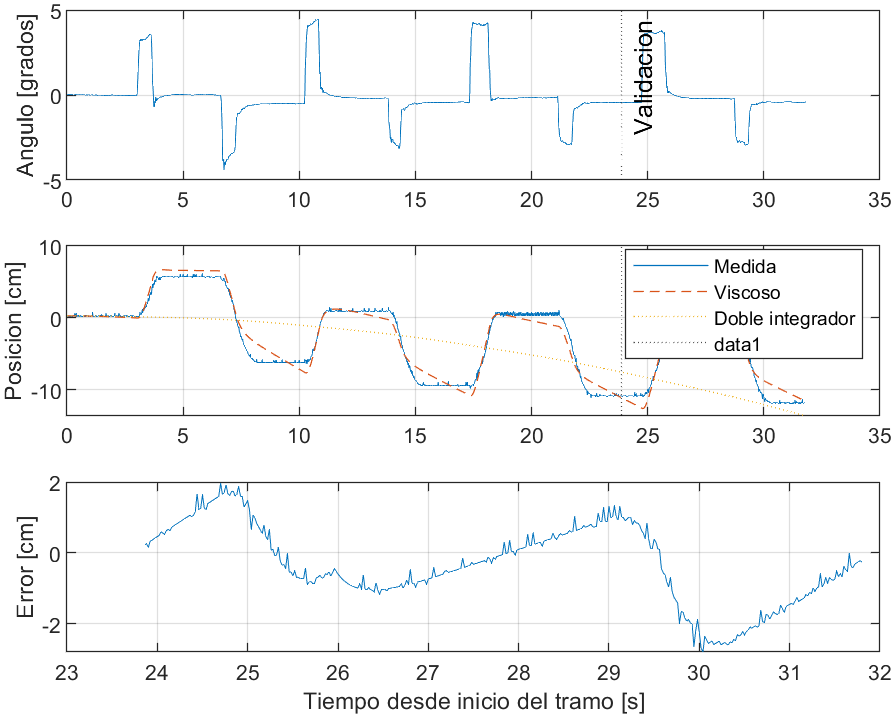
\includegraphics[width=1\textwidth]{imagenes/identificacion-del-carrito.png}
        \caption{Comparación entre la posición medida del carrito y la estimada por el modelo a partir del ángulo registrado. Ambas posiciones utilizan la referencia $y=d-15.612\,\text{cm}$.}
        \label{fig:carrito_posicion_medida_estimada}
    \end{figure}

    El doble integrador obtuvo menor RMSE y mejor FIT que el modelo con rozamiento viscoso en este tramo de validación. Ambos FIT fueron negativos, por lo que ninguno logró predecir la posición mejor que una posición constante igual a la media del tramo. Por lo tanto, estas métricas no permiten afirmar que el modelo viscoso sea el más preciso.

    Se cree que el error puede deberse, en parte, a que el rozamiento real no es solamente proporcional a la velocidad: pueden intervenir fricción estática, cambios de sentido y pequeñas irregularidades del montaje. También pueden contribuir el ruido de los sensores y los errores en el ángulo utilizado como entrada. Además, la simulación no corrige su posición con las mediciones: pequeñas diferencias de aceleración pueden acumularse y producir diferencias importantes de posición. Estas son posibles explicaciones, no causas comprobadas con este ensayo.

    Aún con estas limitaciones, se decidió conservar el modelo con rozamiento viscoso como punto de partida para el diseño, porque representa de manera sencilla una resistencia al movimiento que el doble integrador no contempla. La elección no se basa en que haya obtenido el mejor FIT, sino en disponer de una aproximación física simple con la cual comenzar el trabajo. En las pruebas realizadas con controladores P, PI y PID se logró estabilizar el carrito, lo que muestra que una aproximación de la planta puede resultar útil para controlar aunque no prediga exactamente la posición. 

    Al controlar con realimentación, se mide continuamente la posición y se actúa para reducir su diferencia con la referencia. Esto permite tolerar ciertos errores del modelo y ayuda a explicar por qué un ajuste imperfecto puede servir para el diseño.

    La estabilidad observada no implica que las respuestas reales coincidan exactamente con las simuladas. Pueden existir diferencias en las oscilaciones, el sobrepico, el tiempo de establecimiento o el error final. Estas diferencias se analizarán en la sección de diseño y evaluación de los controladores, comparando las respuestas simuladas con las experimentales.
   
     \subsection{Modelo de la planta completa}
        \subsubsection{Transferencia entrada--salida}
    La planta completa reúne los dos modelos obtenidos: el servo convierte el comando en una inclinación de la barra y esa inclinación produce el movimiento del carrito. Como la salida del primer modelo es la entrada del segundo, sus transferencias se multiplican:
    \[
        G_P(s)=G_s(s)G_c(s),\qquad
        G_s(s)=\frac{87.92}{s^2+91.07s+2310},\qquad
        G_c(s)=\frac{19.619739}{s(s+5.7317425)}.
    \]
    La entrada es la variación del comando del servo respecto de la horizontal, $\Delta u=u-u_0$, en microsegundos, con $u_0=1544\,\mu\text{s}$. La salida es la variación de posición del carrito respecto de una referencia fija, expresada en centímetros. Con los últimos parámetros del carrito y los coeficientes redondeados del servo, el modelo de trabajo resulta:
    \begin{equation}
        G_P(s)=\frac{\Delta Y(s)}{\Delta U(s)}
        =\frac{87.92\cdot19.619739}
        {(s^2+91.07s+2310)\,s(s+5.7317425)}.
        \label{eq:planta_completa}
    \end{equation}
    El ángulo intermedio se expresa en grados en ambos modelos: no corresponde aplicar nuevamente un factor de conversión de grados a radianes ni multiplicar por la gravedad. La planta tiene un polo en el origen y tres polos con parte real negativa; no es asintóticamente estable en lazo abierto.

    Esta transferencia representa solamente la parte lineal del modelo. El término constante $c=-3.2630965\,\text{cm/s}^2$ se utilizó para ajustar y validar el movimiento registrado, pero no forma parte de la transferencia comando--posición. Por eso, para reproducir aquel ensayo en una simulación, se debe agregar ese término a la ecuación de aceleración del carrito y utilizar $y(0)=0.2995\,\text{cm}$ y $\dot y(0)=0$. La transferencia por sí sola, con condiciones iniciales nulas, no reproduce la misma simulación utilizada para calcular el RMSE y el FIT.

    \subsubsection{Representación en variables de estado}
    Una realización de la parte lineal sin retardo se obtiene con
    $x=[\delta y\;\delta\dot y\;\delta\theta_b\;\delta\dot\theta_b]^\mathsf{T}$:
    \begin{equation}
        \dot x=Ax+B\delta u,\qquad \delta y=Cx+D\delta u,
    \end{equation}
    \[
        A=\begin{bmatrix}
            0&1&0&0\\
            0&-5.7317425&19.619739&0\\
            0&0&0&1\\
            0&0&-2310&-91.07
        \end{bmatrix},\quad
        B=\begin{bmatrix}0\\0\\0\\87.92\end{bmatrix},\quad
        C=\begin{bmatrix}1&0&0&0\end{bmatrix},\quad D=0.
        \label{eq:estados_planta}
    \]

    Las unidades de los estados son, respectivamente, cm, cm/s, grados y grados/s. La segunda fila de $A$ describe el movimiento del carrito con los nuevos valores de $a_c$ y $K_c$; la cuarta fila y $B$ describen la respuesta del servo. Esta representación omite el término constante $c$, al igual que la transferencia anterior. Si se conserva el sesgo en las coordenadas originales, debe agregarse a la ecuación de estados el vector $[0\;c\;0\;0]^\mathsf{T}$.

    El modelo lineal se adopta como aproximación de trabajo próxima a la horizontal. El sesgo ajustado implica que la horizontal no es un equilibrio exacto del modelo que incluye $c$: para reposo, ese modelo exige $\theta_{b,e}=-c/K_c\simeq0.1663\degree$. Este valor es una consecuencia del ajuste, no una nueva calibración de la horizontal. La referencia de posición utilizada es la definida experimentalmente y no una medición del centro geométrico exacto.

    \subsubsection{Alternativa con retardo fijo}
    La alternativa exigida para el servo conserva sus polos y ganancia y agrega solamente un retardo. En la planta completa resulta
    \[
        G_{P,T_d}(s)=G_P(s)e^{-T_ds}.
    \]
    La comparación se realizó con el script \texttt{TP2/comparar\_retardo\_planta.m} y el registro \texttt{mediciones\_dinamica\_carrito\_2.mat}, que incluye el comando aplicado al servo, el ángulo medido y la distancia del carrito. Se utilizaron las primeras 1733 muestras, entre $0$ y $34.640\,\text{s}$. Se simularon las opciones sin retardo y con retardos fijos de $20$ y $40\,\text{ms}$, manteniendo los mismos parámetros, el término $c$ y las mismas condiciones iniciales. El servo se inició con el ángulo de la primera medición y velocidad angular nula; antes del registro se supuso comando horizontal. Los retardos se implementaron desplazando el comando una o dos muestras, respectivamente, sin utilizar Padé.

    Las métricas de posición se calcularon sobre las últimas 434 muestras, sin reajustar los modelos:
    \begin{center}
    \begin{tabular}{rrr}
        \toprule
        Retardo [ms] & RMSE [cm] & FIT [\%] \\
        \midrule
        0  & 16.67868 & -713.04 \\
        20 & 16.65136 & -711.71 \\
        40 & 16.62408 & -710.38 \\
        \bottomrule
    \end{tabular}
    \end{center}

    \begin{figure}[htbp]
        \centering
        % Reemplazar el recuadro por la imagen y descomentar:
        % \includegraphics[width=0.95\textwidth]{imagenes/comparacion_retardo_planta.png}
        \fbox{\parbox[c][6cm][c]{0.85\textwidth}{\centering
            Espacio para la comparación de la planta completa:\\
            comando, ángulo y posición, con y sin retardo.}}
        \caption{Respuesta medida y simulada de la planta completa para retardos de 0, 20 y 40 ms, con los mismos parámetros y condiciones iniciales.}
        \label{fig:comparacion_retardo_planta}
    \end{figure}

    Las curvas simuladas reproducen parte de las subidas y bajadas observadas, pero presentan una separación de posición que aumenta durante el ensayo. No se trata solamente de un desplazamiento constante que pueda corregirse moviendo la curva: existe una deriva acumulada. Una posible explicación es que pequeñas diferencias entre el ángulo medido y el calculado por el modelo del servo se acumulan al obtener la posición. En el modelo del carrito, una diferencia angular constante $\Delta\theta$ produce, después del transitorio, una diferencia de velocidad $\Delta v=(K_c/a_c)\Delta\theta\simeq3.42\Delta\theta$, con el ángulo en grados y la velocidad en cm/s. Por eso, diferencias angulares pequeñas pueden generar varios centímetros de error durante el registro.

    También pueden contribuir efectos de rozamiento no representados y el hecho de que $c$ se ajustó utilizando el ángulo medido, mientras que aquí se utiliza el ángulo simulado por el servo. Estas explicaciones son hipótesis compatibles con los resultados, no causas identificadas por separado. Se conservaron las predicciones originales, sin desplazar ni quitar tendencias a las curvas para mejorar las métricas. Además, se utilizó la misma corrida que para identificar el carrito; esta comparación no constituye una validación con un ensayo independiente.

    El retardo de $40\,\text{ms}$ obtuvo el menor RMSE, pero la reducción respecto de la opción sin retardo fue de apenas $0.05460\,\text{cm}$, aproximadamente un $0.33\,\%$. La mejora es pequeña frente al error total y no corrige la deriva. Por este motivo se eligió continuar con la planta sin retardo adicional como modelo nominal de trabajo, por su simplicidad y porque el retardo tampoco mejoró la comparación previa comando--ángulo. Esta elección no implica que la planta completa haya quedado validada con precisión: se adopta como punto de partida para el diseño y su utilidad se evaluará mediante las respuestas de los controladores. Un eventual uso posterior de Padé deberá indicar qué retardo se representa y evitar contabilizar dos veces el mismo efecto. El retardo puro no está incluido en la realización de cuatro estados anterior.

    \subsubsection{Ventajas y limitaciones del modelado experimental}
    La identificación por subsistemas permite obtener una representación sencilla sin medir masas, inercias ni geometría detallada, y separar la respuesta del actuador de la del carrito. A cambio, los parámetros dependen del montaje, del rango de excitación, de la calibración y de los sensores utilizados. El modelo lineal no representa explícitamente fricción estática o de Coulomb, holguras, saturaciones ni fallos de eco. Su uso se limita a movimientos próximos a las condiciones ensayadas y debe contrastarse con nuevos ensayos antes de generalizar sus predicciones.

    \section{Limitaciones de diseño}
    La transferencia obtenida del sistema no presenta singularidades en el semiplano derecho, con lo cual no impone cotas inferiores o superiores a la frecuencia de cruce $w_{gc}$. Sin embargo, el ancho de banda del lazo de control se encuentra limitado principalmente por la frecuencia de muestreo y control de $50$ Hz. Dado que no se puede controlar un sistema a una frecuencia mayor a la que se obtienen nuevos datos de los sensores, la dinámica del lazo deberá permanecer por debajo de este valor.

    Por otro lado, a la hora de diseñar los controladores deberá tenerse en consideración que la acción de control no se sature respecto de los límites establecidos previamente, de manera que $u \in [1100 \ \mu\text{s}; 2000 \ \mu\text{s}]$. Para ello se deberá ajustar la ganancia de los controladores a un valor acorde que no provoque acciones de control demasidado violentas.\\

    En cuanto al diseño existe también una relación de compromiso entre la velocidad de respuesta y la robustez y estabilidad del lazo. Generalmente, para alcanzar una mayor velocidad de respuesta se requiere una $w_{gc}$ mayor, lo cual implica aumentar la ganancia del controlador. Pero esto a su vez implica que tanto el margen de fase como el de ganancia disminuirán, debido a la ganancia extra, lo cual degrada la estabilidad del sistema y vuelve al lazo menos robusto ante perturbaciones. Así mismo, una mayor ganancia de controlador suele implicar acciones de control más violentas, lo cual puede ocasionar que la misma exceda los límites permitidos, potencialmente dañando alguno de los actuadores o componentes del sistema.

    \section{Diseño de controladores}

    \subsection{Análisis de los márgenes de la planta}
    Antes de diseñar los controladores se analizó el diagrama de Bode de la planta nominal $G_P(s)$ dada en la ecuación~\ref{eq:planta_completa}, sin retardo adicional. Para realimentación negativa unitaria y ganancia de controlador igual a uno, se obtuvo un margen de fase de $88.4\degree$ a la frecuencia de cruce de ganancia $\omega_{gc}=0.13\,\text{rad/s}$. El margen de ganancia fue de $46.6\,\text{dB}$, a la frecuencia de cruce de fase $\omega_{pc}=11.7\,\text{rad/s}$.

    El margen de retardo obtenido fue de $11.4\,\text{s}$: representa el retardo puro adicional que llevaría al lazo al límite de estabilidad, manteniendo la ganancia considerada. Estos resultados muestran márgenes amplios, aunque con una frecuencia de cruce de ganancia baja, lo que motiva aumentar la ganancia para obtener una respuesta más rápida.

    \begin{figure}[H]
        \centering
        % Reemplazar el recuadro por la imagen y descomentar:
        % \includegraphics[width=0.95\textwidth]{imagenes/bode_planta.png}
        \fbox{\parbox[c][6cm][c]{0.85\textwidth}{\centering
            Espacio para el diagrama de Bode de la planta\\
            con sus márgenes de estabilidad.}}
        \caption{Diagrama de Bode de la planta nominal $G_P(s)$ y márgenes para realimentación negativa unitaria con ganancia de controlador igual a uno.}
        \label{fig:bode_planta}
    \end{figure}

    \subsection{Control proporcional}
    Para el controlador proporcional se adoptó $C_P(s)=K_p$. Como una ganancia positiva constante no modifica la fase, se buscó en el Bode de la planta la frecuencia para la cual la fase fuera aproximadamente $-120\degree$, correspondiente a un margen de fase deseado de $60\degree$. Esta condición se encontró alrededor de $\omega=2.54\,\text{rad/s}$.

    Para desplazar el cruce de ganancia hacia esa región se eligió una ganancia de $26\,\text{dB}$, calculada en MATLAB mediante \texttt{db2mag(26)}:
    \begin{equation}
        K_p=10^{26/20}\simeq19.95\,\frac{\mu\text{s}}{\text{cm}},
        \qquad C_P(s)=K_p.
        \label{eq:controlador_proporcional}
    \end{equation}
    Las unidades corresponden a la entrada incremental del servo en microsegundos y al error de posición en centímetros utilizados en el modelo.

    Al evaluar el lazo abierto compensado $L_P(s)=K_pG_P(s)$, se obtuvo una frecuencia de cruce de ganancia de $2.39\,\text{rad/s}$, con un margen de fase de $61.9\degree$ y un margen de ganancia de $20.6\,\text{dB}$. La ganancia elegida aproxima el objetivo de diseño y conserva un margen de fase ligeramente superior a $60\degree$. Frente al caso de ganancia unitaria, aumenta la frecuencia de cruce a costa de reducir los márgenes de estabilidad.

    \begin{figure}[H]
        \centering
        % Reemplazar el recuadro por la imagen y descomentar:
        % \includegraphics[width=0.95\textwidth]{imagenes/bode_control_proporcional.png}
        \fbox{\parbox[c][6cm][c]{0.85\textwidth}{\centering
            Espacio para el diagrama de Bode de $K_pG_P(s)$\\
            con el controlador proporcional de $26\,\text{dB}$.}}
        \caption{Diagrama de Bode del lazo abierto con control proporcional: $\omega_{gc}=2.39\,\text{rad/s}$, margen de fase de $61.9\degree$ y margen de ganancia de $20.6\,\text{dB}$.}
        \label{fig:bode_control_proporcional}
    \end{figure}

    \subsubsection{Respuesta continua al escalón}
    Con realimentación negativa unitaria, la transferencia entre referencia y posición es
    \[
        T_P(s)=\frac{K_pG_P(s)}{1+K_pG_P(s)}.
    \]
    Para un escalón de referencia de $0.1\,\text{m}=10\,\text{cm}$, el modelo continuo lineal presentó un tiempo de establecimiento al $2\,\%$ de $1.6116\,\text{s}$, un tiempo de subida del $10$ al $90\,\%$ de $0.5295\,\text{s}$ y un tiempo al pico de $1.1295\,\text{s}$. El sobrepaso fue de $6.25\,\%$, equivalente a una posición máxima de $10.625\,\text{cm}$. El valor pico $1.0625$ informado por \texttt{stepinfo(T)} corresponde a un escalón unitario; al multiplicar la referencia por diez, se escala la amplitud de la respuesta, mientras que estos tiempos y el sobrepaso porcentual se mantienen para el modelo lineal.

    \subsubsection{Discretización bilineal y ley de control}
    Se utilizó un período de muestreo $T_s=0.02\,\text{s}$, correspondiente a $50\,\text{Hz}$. Aplicando la transformación bilineal o de Tustin,
    \[
        s=\frac{2}{T_s}\frac{z-1}{z+1},
    \]
    el controlador proporcional conserva su forma, ya que no depende de $s$:
    \begin{equation}
        C_P(z)=K_p=19.95262315,\qquad
        \Delta u[k]=K_p e[k],\qquad e[k]=r[k]-y[k].
        \label{eq:p_discreto}
    \end{equation}
    En este caso $K_i=K_d=0$ y no se utiliza filtro derivativo ($T_f=0$). Para la estructura de ecuación en diferencias utilizada por el programa de Arduino, los coeficientes son $A_1=A_2=B_1=B_2=0$ y $B_0=19.95262315$.

    El comando absoluto se calcula sumando el pulso de equilibrio, limitando el resultado al intervalo operativo y redondeando a microsegundos enteros:
    \[
        u[k]=\operatorname{round}\!\left(
        \operatorname{sat}_{[1100,2000]}\left(1544+K_p e[k]\right)\right)
        \quad [\mu\text{s}],
    \]
    con el error expresado en centímetros. Esta es la ley utilizada en la simulación de la implementación digital.

    Para simular la planta muestreada se utilizó una discretización con retenedor de orden cero (ZOH), que representa el comando constante entre actualizaciones del Arduino. La transformación bilineal se aplica al controlador. Se verificó en MATLAB que tanto el lazo continuo como el lazo digital lineal tienen sus polos en la región de estabilidad correspondiente. Esta comprobación se refiere a los modelos nominales sin saturación ni redondeo.

    \subsubsection{Simulación digital del escalón de posición}
    Se simuló un escalón de $10\,\text{cm}$ aplicado en $t=2\,\text{s}$, partiendo del reposo y de posición cero. Se tomó el modelo nominal sin el sesgo de aceleración ($c=0$), incluyendo los límites y el redondeo del comando. Los resultados se resumen en la Tabla~\ref{tab:p_escalon_simulado}; el tiempo de establecimiento se mide desde la aplicación del escalón.

    \begin{table}[H]
        \centering
        \caption{Respuesta simulada al escalón de $10\,\text{cm}$ con control proporcional digital, límites y redondeo del comando.}
        \label{tab:p_escalon_simulado}
        \begin{tabular}{lr}
            \toprule
            Magnitud & Resultado \\
            \midrule
            Tiempo de establecimiento al $2\,\%$ & $1.6190\,\text{s}$ \\
            Sobrepaso máximo & $7.28\,\%$ \\
            Error medio en los últimos $2\,\text{s}$ & $-0.00040\,\text{cm}$ \\
            Pulso mínimo / máximo & $1529\,/\,1744\,\mu\text{s}$ \\
            Muestras con saturación & $0$ \\
            \bottomrule
        \end{tabular}
    \end{table}

    El tiempo de establecimiento resulta cercano al continuo y el sobrepaso aumenta de $6.25\,\%$ a $7.28\,\%$. La comparación contempla conjuntamente el muestreo y el redondeo del comando. Durante este ensayo no se alcanzaron los límites del actuador.

    El error estacionario del modelo digital lineal nominal fue numéricamente $-5.3291\times10^{-14}\,\text{cm}$, compatible con cero dentro de la precisión de cálculo. Esto es consistente con el polo en el origen de la planta: con realimentación unitaria estable, el modelo nominal con control P tiene error nulo ante una referencia escalón. El error medio de $-0.00040\,\text{cm}$ corresponde a una ventana final de la simulación con redondeo y no constituye una medición experimental. La fricción, un desajuste del equilibrio u otras perturbaciones pueden producir un error persistente en la planta real, por lo que este resultado deberá contrastarse con el ensayo.

    \begin{figure}[H]
        \centering
        % Reemplazar el recuadro por la imagen y descomentar:
        % \includegraphics[width=0.95\textwidth]{imagenes/p_escalon_simulado.png}
        \fbox{\parbox[c][6cm][c]{0.85\textwidth}{\centering
            Espacio para la respuesta al escalón de $10\,\text{cm}$:\\
            modelos continuo y digital, y comando del servo.}}
        \caption{Respuesta simulada con control P ante un escalón de posición de $10\,\text{cm}$: comparación del modelo continuo, el digital lineal y el digital con límites y redondeo. Se incluye el pulso aplicado al servo.}
        \label{fig:p_escalon_simulado}
    \end{figure}

    \subsubsection{Comparación experimental del escalón de posición}
    Se aplicó a la planta real un escalón de referencia de $0$ a $10\,\text{cm}$ con el controlador proporcional diseñado. El registro se guardó en \texttt{controlador\_proporcional.mat} y se procesó mediante \texttt{comparar\_escalon\_P.m}. La referencia y la distancia recibidas se convirtieron a posiciones relativas restando $15.612\,\text{cm}$. Para superponer las respuestas se tomó como $t=0$ el instante del cambio de referencia, registrado a los $5\,\text{s}$ del ensayo. No se aplicaron desplazamientos de posición para hacer coincidir las curvas.

    La comparación se realizó con la simulación digital nominal, incluyendo el muestreo, los límites y el redondeo del comando, con $c=0$. La Tabla~\ref{tab:p_comparacion_escalon} resume los resultados posteriores al escalón. Se define el error como $e=r-y$ y se calcula su promedio sobre los últimos $2\,\text{s}$ de cada registro.

    \begin{table}[H]
        \centering
        \caption{Comparación de la respuesta real y simulada al escalón de $10\,\text{cm}$ con control P.}
        \label{tab:p_comparacion_escalon}
        \begin{tabular}{lrr}
            \toprule
            Magnitud & Planta real & Simulación digital \\
            \midrule
            Tiempo de establecimiento al $2\,\%$ & No alcanzado & $1.62\,\text{s}$ \\
            Sobrepaso máximo & $81.91\,\%$ & $7.28\,\%$ \\
            Error medio final & $-0.952\,\text{cm}$ & $-0.00040\,\text{cm}$ \\
            Pulso mínimo & $1381\,\mu\text{s}$ & $1529\,\mu\text{s}$ \\
            Pulso máximo & $1753\,\mu\text{s}$ & $1744\,\mu\text{s}$ \\
            \bottomrule
        \end{tabular}
    \end{table}

    \begin{figure}[H]
        \centering
        % Reemplazar el recuadro por la imagen y descomentar:
        % Imagen generada por el script: TP2/comparacion_escalon_P.png.
        % \includegraphics[width=0.95\textwidth]{../comparacion_escalon_P.png}
        \fbox{\parbox[c][7cm][c]{0.85\textwidth}{\centering
            Espacio para la comparación del escalón con control P:\\
            referencia, posición real y simulada,\\
            y pulsos aplicados al servo.}}
        \caption{Comparación de la respuesta real y simulada al escalón de $10\,\text{cm}$ con control proporcional. El origen temporal corresponde al cambio de referencia. Se muestran la posición del carrito y el comando del servo.}
        \label{fig:p_comparacion_escalon}
    \end{figure}

    La planta real presentó una oscilación considerablemente mayor que la simulada: alcanzó aproximadamente $18.19\,\text{cm}$, frente a los $10\,\text{cm}$ de referencia. Luego del transitorio, la posición media en los últimos $2\,\text{s}$ fue de aproximadamente $10.95\,\text{cm}$, mientras que la simulación convergió prácticamente a la referencia. El registro real no permaneció dentro de la banda de establecimiento de $10\pm0.2\,\text{cm}$ hasta el final del ensayo, por lo que no se obtuvo un tiempo de establecimiento con ese criterio durante los $9.02\,\text{s}$ posteriores al escalón.

    En ambos casos los pulsos permanecieron dentro del intervalo permitido de $[1100,2000]\,\mu\text{s}$. Por lo tanto, el mayor sobrepaso observado no se explica por una saturación del comando registrado. Los resultados muestran que el modelo nominal subestima el sobrepaso y no reproduce el desplazamiento final de la planta real. Entre las posibles causas se encuentran el rozamiento no representado, las diferencias entre la dinámica real y la identificada, y un desajuste del punto de equilibrio; este ensayo no permite distinguir sus contribuciones por separado.

    El error medio final real evidencia una diferencia persistente respecto de la consigna en la ventana observada, aunque la duración del registro no permite asegurar que sea el error de estado estacionario definitivo. Este resultado se utilizará como referencia para evaluar si la incorporación de acción integral reduce el error final respecto del controlador proporcional.

    \subsubsection{Simulación de una perturbación impulsiva sobre el carrito}
    Para representar un ligero golpe se mantuvo la referencia en cero y se introdujo en $t=5\,\text{s}$ un salto de velocidad de $5.00\,\text{cm/s}$. Esta perturbación representa el efecto de un impulso mecánico sobre el carrito; no es un impulso en la referencia de posición. La amplitud elegida es ilustrativa, ya que no se dispone de una medición del impulso aplicado en el ensayo real.

    Con el mismo controlador digital y $c=0$, el máximo desplazamiento absoluto posterior al golpe fue de $0.61569\,\text{cm}$. El pulso del servo permaneció entre $1532$ y $1545\,\mu\text{s}$, sin muestras saturadas. Estos resultados describen la recuperación simulada para el salto de velocidad elegido.

    \begin{figure}[H]
        \centering
        % Reemplazar el recuadro por la imagen y descomentar:
        % \includegraphics[width=0.95\textwidth]{imagenes/p_golpe_simulado.png}
        \fbox{\parbox[c][6cm][c]{0.85\textwidth}{\centering
            Espacio para la recuperación simulada ante el golpe:\\
            posición del carrito y comando del servo.}}
        \caption{Respuesta simulada con control P digital ante un salto de velocidad de $5\,\text{cm/s}$ en $t=5\,\text{s}$, con referencia de posición nula.}
        \label{fig:p_golpe_simulado}
    \end{figure}

    \subsubsection{Comparación experimental ante un golpe}
    Con la referencia fija en cero se aplicó un ligero golpe al carrito y se guardó el ensayo en \texttt{controlador\_proporcional\_golpe.mat}. La comparación se realizó mediante \texttt{comparar\_golpe.m}, tomando como inicio de la perturbación $t=2.089\,\text{s}$ del registro original. Para representar el sentido del movimiento observado, en esta comparación se utilizó un salto de velocidad simulado de $-5\,\text{cm/s}$, dirigido hacia el sensor. Su amplitud es ilustrativa y no corresponde a una medición de la intensidad del golpe real.

    El máximo desplazamiento absoluto respecto de la referencia fue de $6.188\,\text{cm}$ en la planta real y de $0.61569\,\text{cm}$ en la simulación. El modelo simulado recuperó la banda de $\pm0.2\,\text{cm}$ en $0.78\,\text{s}$, mientras que el registro real no permaneció en esa banda hasta el final del ensayo. El error medio en los últimos $2\,\text{s}$ fue de $-0.58347\,\text{cm}$ en la planta real y de aproximadamente $-0.00055\,\text{cm}$ en la simulación. Los pulsos permanecieron entre $1504$ y $1667\,\mu\text{s}$ en el ensayo, y entre $1543$ y $1556\,\mu\text{s}$ en la simulación, sin alcanzar los límites en ninguno de los casos.

    \begin{figure}[H]
        \centering
        % Reemplazar el recuadro por la imagen y descomentar:
        % \includegraphics[width=0.95\textwidth]{../comparacion_golpe_P.png}
        \fbox{\parbox[c][7cm][c]{0.85\textwidth}{\centering
            Espacio para la comparación ante un golpe con control P:\\
            posición real y simulada, y comando del servo.}}
        \caption{Respuesta real y simulada con control proporcional ante una perturbación sobre el carrito, con referencia nula. El origen temporal corresponde al inicio seleccionado del golpe; la amplitud del impulso real no está medida.}
        \label{fig:p_comparacion_golpe}
    \end{figure}

    La planta real regresó hacia la zona de referencia tras la perturbación, aunque conservó un desplazamiento final. Antes del golpe, la mediana de posición en el primer segundo ya era de $0.6409\,\text{cm}$; este desplazamiento se mantuvo en las curvas, sin corregirlo. Por lo tanto, el error final no puede atribuirse solamente al golpe. La comparación es cualitativa, ya que difieren tanto la condición inicial de posición como la intensidad de la perturbación: la diferencia entre los máximos no permite cuantificar por sí sola el error del modelo. El desplazamiento persistente observado, también presente en el ensayo de escalón, motiva evaluar la incorporación de acción integral.

    \subsection{Control proporcional-integral}
    Para reducir el error persistente observado con el control proporcional se propone incorporar una acción integral:
    \begin{equation}
        C_{PI}(s)=K_p+\frac{K_i}{s}.
        \label{eq:controlador_pi}
    \end{equation}
    La integral acumula el error y permite mantener una corrección aun cuando este se reduce; un valor excesivo de $K_i$ puede aumentar las oscilaciones y reducir los márgenes de estabilidad. Para la sintonía se eligió un cero en $s=-0.5\,\text{rad/s}$ y una ganancia proporcional de $22\,\text{dB}$, inferior a la utilizada en el P:
    \begin{equation}
        C_{PI}(s)=10^{22/20}\frac{s+0.5}{s}
        =12.589254+\frac{6.294627}{s}.
        \label{eq:pi_sintonia}
    \end{equation}
    Por lo tanto, $K_p=12.589254\,\mu\text{s}/\text{cm}$ y $K_i=6.294627\,\mu\text{s}/(\text{cm}\,\text{s})$. La reducción de la ganancia proporcional acompaña la incorporación de la integral, teniendo en cuenta el elevado sobrepaso observado en la planta real con el P.

    \subsubsection{Márgenes de estabilidad y respuesta continua}
    Para el lazo abierto compensado $L_{PI}(s)=C_{PI}(s)G_P(s)$ se obtuvo un margen de fase de $53\degree$ a la frecuencia de cruce de ganancia $\omega_{gc}=1.65\,\text{rad/s}$, y un margen de ganancia de $23.7\,\text{dB}$ a la frecuencia de cruce de fase $\omega_{pc}=11.1\,\text{rad/s}$. Frente al P diseñado, disminuyen tanto la frecuencia de cruce como el margen de fase, mientras que aumenta el margen de ganancia.

    \begin{figure}[H]
        \centering
        % Reemplazar el recuadro por la captura del Bode continuo del PI:
        % \includegraphics[width=0.95\textwidth]{imagenes/bode_control_pi.png}
        \fbox{\parbox[c][6cm][c]{0.85\textwidth}{\centering
            Espacio para el Bode de $C_{PI}(s)G_P(s)$\\
            con los márgenes de estabilidad.}}
        \caption{Diagrama de Bode del lazo abierto con control PI: margen de fase de $53\degree$ y margen de ganancia de $23.7\,\text{dB}$.}
        \label{fig:bode_control_pi}
    \end{figure}

    La respuesta continua a un escalón de $10\,\text{cm}$ presentó un tiempo de establecimiento al $2\,\%$ de $5.1873\,\text{s}$, un tiempo de subida del $10$ al $90\,\%$ de $0.6570\,\text{s}$ y un tiempo al pico de $1.8011\,\text{s}$. El sobrepaso fue de $23.75\,\%$, equivalente a una posición máxima de $12.375\,\text{cm}$. El pico de $1.2375$ informado por \texttt{stepinfo(T)} corresponde al escalón unitario. Estos resultados muestran una respuesta nominal más lenta y con mayor sobrepaso que la del P; la incorporación de integral busca mejorar la corrección del error persistente real, y no implica por sí sola una mejora del transitorio.

    \subsubsection{Discretización bilineal}

    Con el mismo período $T_s=0.02\,\text{s}$, la transformación bilineal resulta en
    \[
        C_{PI}(z)=K_p+\frac{K_iT_s}{2}\frac{z+1}{z-1},
    \]
    cuya ecuación en diferencias, antes de aplicar los límites del actuador, es
    \begin{equation}
        \Delta u[k]=\Delta u[k-1]
        +\left(K_p+\frac{K_iT_s}{2}\right)e[k]
        +\left(-K_p+\frac{K_iT_s}{2}\right)e[k-1].
        \label{eq:pi_discreto}
    \end{equation}
    Esta expresión permite utilizar la misma estructura del programa de Arduino, con $A_1=1$, $A_2=B_2=0$, $B_0=K_p+K_iT_s/2$ y $B_1=-K_p+K_iT_s/2$. Para las ganancias elegidas se obtiene
    \[
        C_{PI}(z)=\frac{12.6522004-12.5263078z^{-1}}{1-z^{-1}},
    \]
    y la ecuación en diferencias queda
    \[
        \Delta u[k]=\Delta u[k-1]+12.6522004e[k]-12.5263078e[k-1].
    \]
    Los coeficientes para Arduino son entonces $A_1=1$, $A_2=0$, $B_0=12.6522004$, $B_1=-12.5263078$ y $B_2=0$. Se verificó en MATLAB la estabilidad de los lazos continuo y digital lineales nominales.

    \subsubsection{Simulación digital del escalón de posición}
    Con el script \texttt{disenar\_control.m} se simuló un escalón de $0$ a $10\,\text{cm}$ en $t=2\,\text{s}$, partiendo del reposo y de posición cero, con $c=0$. La planta se discretizó con ZOH y el controlador con Tustin. Se incluyeron la saturación del pulso a $[1100,2000]\,\mu\text{s}$ y el redondeo a microsegundos enteros. La recurrencia utiliza la salida limitada, sin redondear, como memoria del controlador, de la misma manera que el programa de Arduino.

    \begin{table}[H]
        \centering
        \caption{Respuesta simulada al escalón de $10\,\text{cm}$ con control PI digital, límites y redondeo.}
        \label{tab:pi_escalon_simulado}
        \begin{tabular}{lr}
            \toprule
            Magnitud & Resultado \\
            \midrule
            Tiempo de establecimiento al $2\,\%$ & $5.1527\,\text{s}$ \\
            Sobrepaso máximo & $24.42\,\%$ \\
            Error medio en los últimos $2\,\text{s}$ & $-0.00040\,\text{cm}$ \\
            Pulso mínimo / máximo & $1535\,/\,1675\,\mu\text{s}$ \\
            Muestras con saturación & $0$ \\
            \bottomrule
        \end{tabular}
    \end{table}

    La respuesta digital conserva un comportamiento cercano al continuo: el establecimiento es de aproximadamente $5.15\,\text{s}$ y el sobrepaso aumenta a $24.42\,\%$, sin alcanzar los límites del actuador. El error estacionario del modelo digital lineal fue numéricamente $-1.5543\times10^{-14}\,\text{cm}$, compatible con cero. Como el modelo nominal con P ya tenía error nulo al escalón, esta simulación con $c=0$ no demuestra una mejora del error final por la integral. Su efecto sobre el desplazamiento persistente observado deberá evaluarse con el ensayo real.

    \begin{figure}[H]
        \centering
        % Imagen generada por disenar_control.m: TP2/PI_escalon_simulado.png.
        % Reemplazar el recuadro y descomentar:
        % \includegraphics[width=0.95\textwidth]{../PI_escalon_simulado.png}
        \fbox{\parbox[c][7cm][c]{0.85\textwidth}{\centering
            Espacio para el escalón simulado con PI:\\
            comparación continua y digital,\\
            y pulso aplicado al servo.}}
        \caption{Respuesta simulada con control PI ante un escalón de posición de $10\,\text{cm}$: modelos continuo, digital lineal y digital con límites y redondeo, junto con el comando del servo.}
        \label{fig:pi_escalon_simulado}
    \end{figure}

    \subsubsection{Simulación de una perturbación impulsiva}
    Como evaluación adicional, se mantuvo la referencia en cero y se introdujo un salto de velocidad de $5\,\text{cm/s}$ en $t=5\,\text{s}$, con las mismas condiciones nominales utilizadas para el P. El máximo desplazamiento absoluto posterior al golpe fue de $0.65677\,\text{cm}$. El comando permaneció entre $1535$ y $1545\,\mu\text{s}$, sin muestras saturadas. La amplitud del salto es ilustrativa y permite comparar ambos controladores bajo la misma perturbación simulada.

    \begin{figure}[H]
        \centering
        % Imagen generada por disenar_control.m: TP2/PI_golpe_simulado.png.
        % Reemplazar el recuadro y descomentar:
        % \includegraphics[width=0.95\textwidth]{../PI_golpe_simulado.png}
        \fbox{\parbox[c][7cm][c]{0.85\textwidth}{\centering
            Espacio para el golpe simulado con PI:\\
            posición del carrito y comando del servo.}}
        \caption{Respuesta simulada con control PI digital ante un salto de velocidad de $5\,\text{cm/s}$ en $t=5\,\text{s}$, con referencia nula.}
        \label{fig:pi_golpe_simulado}
    \end{figure}

    \subsubsection{Comparación experimental del escalón de posición}
    Se repitió el ensayo de referencia de $0$ a $10\,\text{cm}$ con el controlador PI implementado en su forma bilineal. El registro se procesó mediante el comparador generalizado \texttt{comparar\_escalon\_P.m}, utilizando $C_{PI}(s)$ de la ecuación~\ref{eq:pi_sintonia}. Se alinearon temporalmente las respuestas en el instante del escalón y se conservaron las posiciones medidas, expresadas respecto de la referencia experimental. No se detectaron muestras inválidas.

    \begin{table}[H]
        \centering
        \caption{Comparación real y simulada del escalón de $10\,\text{cm}$ con control PI. El error final es el promedio de $r-y$ en los últimos $2\,\text{s}$.}
        \label{tab:pi_comparacion_escalon}
        \begin{tabular}{lrr}
            \toprule
            Magnitud & Planta real & Simulación digital \\
            \midrule
            Tiempo de establecimiento al $2\,\%$ & No alcanzado & $5.16\,\text{s}$ \\
            Sobrepaso máximo & $74.40\,\%$ & $24.42\,\%$ \\
            Error medio final & $-0.13321\,\text{cm}$ & $-0.000397\,\text{cm}$ \\
            Pulso mínimo & $1450\,\mu\text{s}$ & $1535\,\mu\text{s}$ \\
            Pulso máximo & $1669\,\mu\text{s}$ & $1675\,\mu\text{s}$ \\
            \bottomrule
        \end{tabular}
    \end{table}

    \begin{figure}[H]
        \centering
        % Imagen generada por el comparador: TP2/comparacion_escalon_PI.png.
        % Reemplazar el recuadro y descomentar:
        % \includegraphics[width=0.95\textwidth]{../comparacion_escalon_PI.png}
        \fbox{\parbox[c][7cm][c]{0.85\textwidth}{\centering
            Espacio para la comparación del escalón con PI:\\
            referencia, posición real y simulada,\\
            y pulsos aplicados al servo.}}
        \caption{Comparación experimental y simulada del escalón de $10\,\text{cm}$ con control PI, con origen temporal en el cambio de referencia. Se incluyen la posición y el comando del servo.}
        \label{fig:pi_comparacion_escalon}
    \end{figure}

    La planta real alcanzó aproximadamente $17.44\,\text{cm}$, por lo que el sobrepaso continuó siendo considerablemente mayor que el previsto por el modelo. El RMSE entre las posiciones real y simulada fue de $1.9019\,\text{cm}$ en el intervalo comparado. Los pulsos registrados y simulados permanecieron dentro de $[1100,2000]\,\mu\text{s}$, por lo que no se observó saturación del comando que explique esta diferencia.

    Respecto del ensayo con P, el sobrepaso real disminuyó de $81.91\,\%$ a $74.40\,\%$, una reducción moderada de $7.51$ puntos porcentuales. La mejora más marcada se observó en el error medio final: su magnitud pasó de $0.952\,\text{cm}$ a $0.13321\,\text{cm}$, aproximadamente un $86\,\%$ menor. La posición media final con PI fue, por tanto, cercana a $10.133\,\text{cm}$. Este resultado es consistente con el efecto esperado de la acción integral sobre un error persistente, aunque entre ambos ensayos también se modificó la ganancia proporcional y no puede atribuirse todo el cambio exclusivamente a la integral.

    A pesar de que el error medio final quedó dentro de $\pm0.2\,\text{cm}$, las muestras reales no permanecieron en esa banda hasta el final del registro; por eso no se obtuvo un tiempo de establecimiento al $2\,\%$. Un promedio pequeño no implica que todas las mediciones cumplan la tolerancia. En consecuencia, el PI mejoró la precisión media final frente al P en los ensayos realizados, pero mantuvo un transitorio con sobrepaso elevado y diferencias importantes respecto de la simulación. El error informado corresponde a la ventana final observada y no garantiza el valor asintótico del error de estado estacionario.

    \subsubsection{Comparación experimental ante un golpe}
    Se mantuvo la referencia en cero y se aplicó un ligero golpe al carrito con el controlador PI activo. El ensayo se procesó mediante \texttt{comparar\_golpe.m}, fijando el inicio de la perturbación en $t=2.771\,\text{s}$ del registro original. Para la comparación se utilizó un salto de velocidad simulado de $-5\,\text{cm/s}$, dirigido hacia el sensor, con el modelo nominal sin sesgo y el controlador discretizado mediante Tustin.

    \begin{table}[H]
        \centering
        \caption{Comparación real y simulada ante un golpe con control PI. La recuperación se evalúa respecto de la banda fija de $\pm0.2\,\text{cm}$ alrededor de la referencia nula.}
        \label{tab:pi_comparacion_golpe}
        \begin{tabular}{lrr}
            \toprule
            Magnitud & Planta real & Simulación digital \\
            \midrule
            Máximo desplazamiento absoluto & $4.6174\,\text{cm}$ & $0.65677\,\text{cm}$ \\
            Tiempo de recuperación a la banda & No alcanzado & $2.26\,\text{s}$ \\
            Error medio en los últimos $2\,\text{s}$ & $-0.79037\,\text{cm}$ & $-0.00055\,\text{cm}$ \\
            Pulso mínimo & $1467\,\mu\text{s}$ & $1543\,\mu\text{s}$ \\
            Pulso máximo & $1637\,\mu\text{s}$ & $1553\,\mu\text{s}$ \\
            Muestras en los límites del comando & $0$ & $0$ \\
            \bottomrule
        \end{tabular}
    \end{table}

    \begin{figure}[H]
        \centering
        % Imagen generada por comparar_golpe(..., 'PI', ...):
        % TP2/comparacion_golpe_PI.png. Reemplazar el recuadro y descomentar:
        % 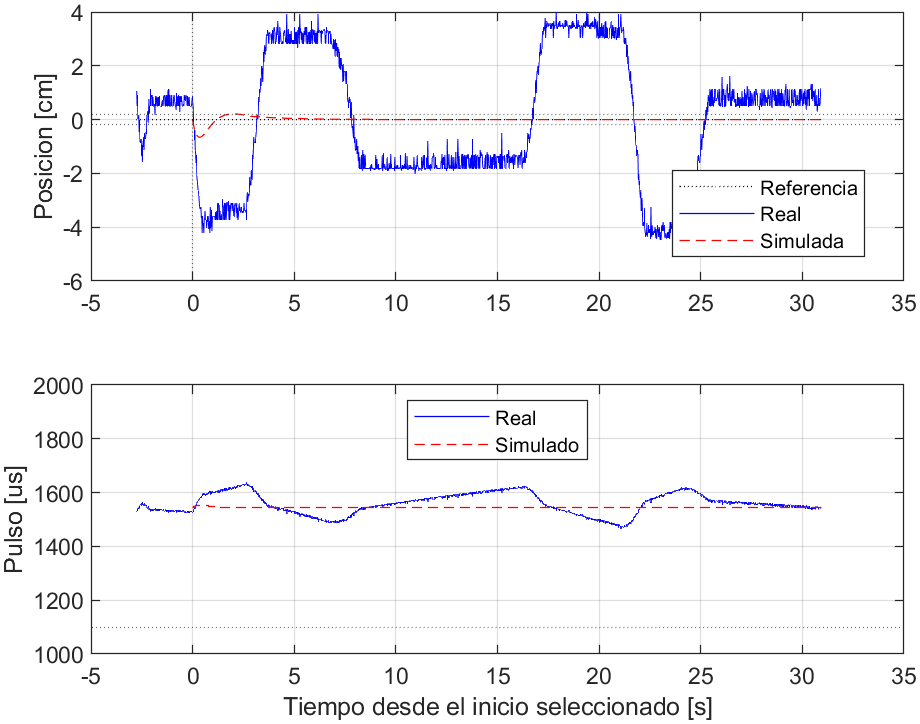
\includegraphics[width=0.95\textwidth]{../comparacion_golpe_PI.png}
        \fbox{\parbox[c][7cm][c]{0.85\textwidth}{\centering
            Espacio para la comparación ante un golpe con PI:\\
            posición real y simulada, y comando del servo.}}
        \caption{Respuesta real y simulada con control PI ante una perturbación sobre el carrito, con referencia nula. El origen temporal corresponde al inicio seleccionado del golpe; la intensidad del impulso real no está medida.}
        \label{fig:pi_comparacion_golpe}
    \end{figure}

    El desplazamiento máximo real fue mayor que el simulado y la respuesta medida no permaneció dentro de la banda de $\pm0.2\,\text{cm}$ hasta el final del registro. El error medio final de $-0.79037\,\text{cm}$ corresponde a una posición media de $0.79037\,\text{cm}$, mientras que la simulación regresó prácticamente a cero. La mediana real del primer segundo era de $0.1629\,\text{cm}$ y se conservó sin corregir las curvas. No se alcanzaron los límites del comando, por lo que la saturación registrada no explica las diferencias observadas.

    A diferencia del ensayo de escalón, en este ensayo el PI no presentó un error medio final menor que el obtenido con P: su magnitud fue de $0.79037\,\text{cm}$ frente a $0.58347\,\text{cm}$. Aunque el máximo desplazamiento real fue menor, las intensidades de los golpes no están medidas y las condiciones iniciales y ventanas de observación difieren; por ello, estos valores no permiten concluir que un controlador rechace mejor la misma perturbación que el otro. En las simulaciones, con igual magnitud del salto de velocidad, el PI recuperó la banda en $2.26\,\text{s}$ frente a $0.78\,\text{s}$ del P.

    El error persistente medido con PI muestra que la mejora observada ante el escalón no se reprodujo en este ensayo de golpe. No puede determinarse su causa solamente con estas métricas: será necesario revisar el registro y la implementación para distinguir entre efectos de la planta, de la medición y del controlador. El promedio final informado describe la ventana observada y no demuestra por sí solo un error de estado estacionario asintótico.

    \subsection{Control proporcional-derivativo}
    Para mejorar el amortiguamiento y reducir las oscilaciones observadas en los ensayos anteriores se diseñó un controlador proporcional-derivativo con filtro. Se eligió un cero en $s=-3\,\text{rad/s}$ y un polo de filtrado en $s=-6\,\text{rad/s}$, con factor de ganancia $10^{24/20}$:
    \begin{equation}
        C_{PD}(s)=10^{24/20}\frac{s+3}{s+6}
        =K_p+\frac{K_ds}{1+T_fs},
        \label{eq:controlador_pd}
    \end{equation}
    donde
    \[
        K_p=7.924466\,\frac{\mu\text{s}}{\text{cm}},\qquad
        K_d=1.320744\,\frac{\mu\text{s}\,\text{s}}{\text{cm}},\qquad
        T_f=0.166667\,\text{s},\qquad K_i=0.
    \]
    El factor $10^{24/20}=15.848932$ corresponde a la ganancia de alta frecuencia de esta transferencia, mientras que su ganancia estática es $K_p$. El filtro limita la ganancia de la acción derivativa a altas frecuencias. Se evaluó esta sintonía buscando una respuesta amortiguada y comandos dentro del intervalo operativo. Los resultados siguientes verifican esa condición para los ensayos simulados, pero no demuestran que se haya alcanzado la mayor rapidez posible entre todas las sintonías admisibles.

    \begin{figure}[H]
        \centering
        % Reemplazar el recuadro por la captura del Bode del PD:
        % \includegraphics[width=0.95\textwidth]{imagenes/bode_control_pd.png}
        \fbox{\parbox[c][6cm][c]{0.85\textwidth}{\centering
            Espacio para el Bode de $C_{PD}(s)G_P(s)$\\
            con sus márgenes de estabilidad.}}
        \caption{Diagrama de Bode del lazo abierto con el controlador PD filtrado.}
        \label{fig:bode_control_pd}
    \end{figure}
    % Pendiente: incorporar los márgenes numéricos del PD de esta sintonía.

    \subsubsection{Respuesta continua al escalón}
    Para un escalón de referencia de $10\,\text{cm}$, la respuesta continua nominal presentó un tiempo de establecimiento al $2\,\%$ de $3.7117\,\text{s}$ y un tiempo de subida del $10$ al $90\,\%$ de $1.9616\,\text{s}$, sin sobrepaso. El valor pico unitario fue de $1.0000$, equivalente a $10\,\text{cm}$ para la referencia utilizada. El tiempo al pico informado por MATLAB fue de $10.9228\,\text{s}$; al no existir un máximo transitorio con sobrepaso, este valor no se interpreta como un pico oscilatorio característico.

    \subsubsection{Discretización bilineal}
    Se aplicó Tustin con $T_s=0.02\,\text{s}$, obteniéndose
    \begin{equation}
        C_{PD}(z)=\frac{15.4003772-14.5032679z^{-1}}
        {1-0.886792453z^{-1}}.
        \label{eq:pd_discreto}
    \end{equation}
    Por lo tanto, antes de limitar el comando, la ecuación en diferencias es
    \[
        \Delta u[k]=0.886792453\Delta u[k-1]
        +15.4003772e[k]-14.5032679e[k-1].
    \]
    Los coeficientes para Arduino son $A_1=0.886792453$, $A_2=0$, $B_0=15.4003772$, $B_1=-14.5032679$ y $B_2=0$. Se verificó que tanto el lazo continuo como el digital lineal nominal son estables.

    \subsubsection{Simulación digital del escalón de posición}
    Se repitió la simulación del escalón de $0$ a $10\,\text{cm}$ en $t=2\,\text{s}$, partiendo del reposo y con $c=0$. Se utilizó la planta discretizada con ZOH y la recurrencia del controlador bilineal, incluyendo los límites y el redondeo del pulso como en el programa de Arduino.

    \begin{table}[H]
        \centering
        \caption{Respuesta simulada al escalón de $10\,\text{cm}$ con control PD digital, límites y redondeo.}
        \label{tab:pd_escalon_simulado}
        \begin{tabular}{lr}
            \toprule
            Magnitud & Resultado \\
            \midrule
            Tiempo de establecimiento al $2\,\%$ & $3.6673\,\text{s}$ \\
            Sobrepaso máximo & $0.00\,\%$ \\
            Error medio en los últimos $2\,\text{s}$ & $0.05693\,\text{cm}$ \\
            Pulso mínimo / máximo & $1544\,/\,1698\,\mu\text{s}$ \\
            Muestras con saturación & $0$ \\
            \bottomrule
        \end{tabular}
    \end{table}

    La respuesta digital mantuvo la ausencia de sobrepaso y un tiempo de establecimiento cercano al continuo. Frente a las simulaciones anteriores, el PD elegido presentó menor sobrepaso que P y PI, aunque su establecimiento fue más lento que el del P y más rápido que el del PI. No se alcanzaron los límites del comando durante el ensayo.

    El error estacionario del modelo digital lineal fue numéricamente $3.5527\times10^{-13}\,\text{cm}$, compatible con cero. En cambio, la simulación con redondeo presentó un error medio final de $0.05693\,\text{cm}$. La cuantización del comando puede sostener pequeños errores: para este PD, con $K_p=7.924466\,\mu\text{s}/\text{cm}$, un error constante inferior a aproximadamente $0.5/K_p=0.0631\,\text{cm}$ puede generar una corrección que se redondea a cero microsegundos respecto del centro. El error obtenido es compatible con ese mecanismo y permanece dentro de la banda de $\pm0.2\,\text{cm}$.

    \begin{figure}[H]
        \centering
        % Imagen generada por disenar_control.m: TP2/PD_escalon_simulado.png.
        % Reemplazar el recuadro y descomentar:
        % \includegraphics[width=0.95\textwidth]{../PD_escalon_simulado.png}
        \fbox{\parbox[c][7cm][c]{0.85\textwidth}{\centering
            Espacio para el escalón simulado con PD:\\
            comparación continua y digital,\\
            y pulso aplicado al servo.}}
        \caption{Respuesta simulada con control PD filtrado ante un escalón de posición de $10\,\text{cm}$: modelos continuo, digital lineal y digital con límites y redondeo, junto con el comando del servo.}
        \label{fig:pd_escalon_simulado}
    \end{figure}

    \subsubsection{Simulación de una perturbación impulsiva}
    Con la referencia fija en cero se introdujo un salto de velocidad de $5\,\text{cm/s}$ en $t=5\,\text{s}$, manteniendo las condiciones nominales de los ensayos simulados anteriores. El máximo desplazamiento absoluto posterior al golpe fue de $0.65679\,\text{cm}$. El pulso permaneció entre $1537$ y $1544\,\mu\text{s}$, sin muestras saturadas. La amplitud del salto es ilustrativa y no constituye una medición del impulso real.

    \begin{figure}[H]
        \centering
        % Imagen generada por disenar_control.m: TP2/PD_golpe_simulado.png.
        % Reemplazar el recuadro y descomentar:
        % \includegraphics[width=0.95\textwidth]{../PD_golpe_simulado.png}
        \fbox{\parbox[c][7cm][c]{0.85\textwidth}{\centering
            Espacio para el golpe simulado con PD:\\
            posición del carrito y comando del servo.}}
        \caption{Respuesta simulada con control PD digital ante un salto de velocidad de $5\,\text{cm/s}$ en $t=5\,\text{s}$, con referencia nula.}
        \label{fig:pd_golpe_simulado}
    \end{figure}


    \subsubsection{Comparación experimental del escalón de posición}
    Se aplicó el escalón de referencia de $0$ a $10\,\text{cm}$ a la planta real con el PD filtrado implementado mediante Tustin. Se utilizó el comparador generalizado \texttt{comparar\_escalon\_P.m}, alineando el instante del escalón y conservando las posiciones medidas sin desplazamientos adicionales. No se detectaron muestras inválidas.

    \begin{table}[H]
        \centering
        \caption{Comparación real y simulada del escalón de $10\,\text{cm}$ con control PD. El error final es el promedio de $r-y$ en los últimos $2\,\text{s}$.}
        \label{tab:pd_comparacion_escalon}
        \begin{tabular}{lrr}
            \toprule
            Magnitud & Planta real & Simulación digital \\
            \midrule
            Tiempo de establecimiento al $2\,\%$ & No alcanzado & $3.68\,\text{s}$ \\
            Sobrepaso máximo & $0\,\%$ & $0\,\%$ \\
            Error medio final & $3.6755\,\text{cm}$ & $0.056927\,\text{cm}$ \\
            Pulso mínimo & $1558\,\mu\text{s}$ & $1544\,\mu\text{s}$ \\
            Pulso máximo & $1692\,\mu\text{s}$ & $1698\,\mu\text{s}$ \\
            \bottomrule
        \end{tabular}
    \end{table}

    \begin{figure}[H]
        \centering
        % Imagen generada por el comparador: TP2/comparacion_escalon_PD.png.
        % Reemplazar el recuadro y descomentar:
        % 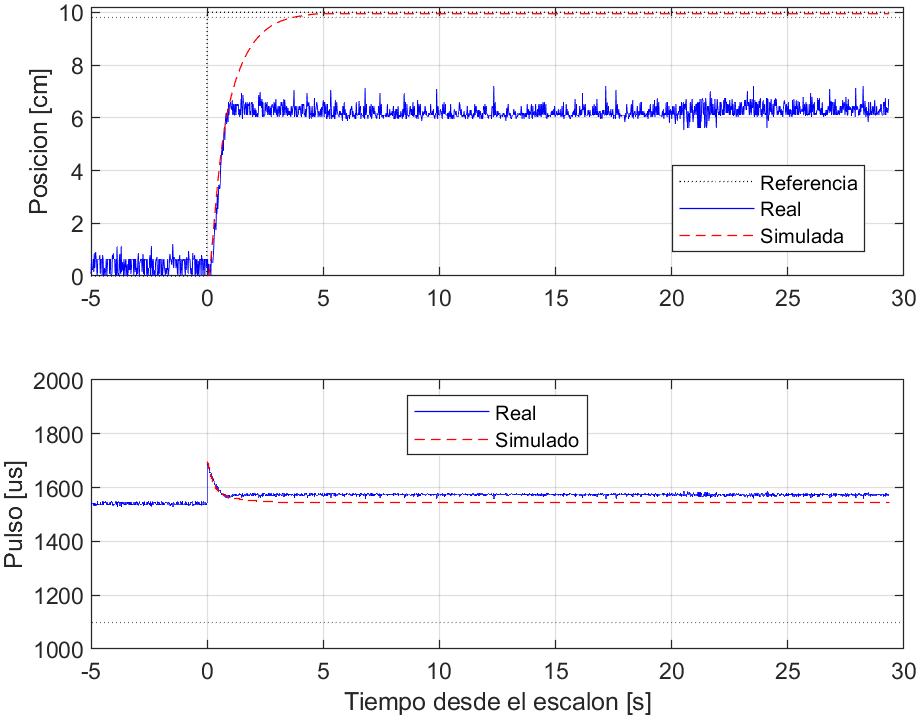
\includegraphics[width=0.95\textwidth]{../comparacion_escalon_PD.png}
        \fbox{\parbox[c][7cm][c]{0.85\textwidth}{\centering
            Espacio para la comparación del escalón con PD:\\
            referencia, posición real y simulada,\\
            y pulsos aplicados al servo.}}
        \caption{Comparación experimental y simulada del escalón de $10\,\text{cm}$ con control PD filtrado. El origen temporal corresponde al cambio de referencia; se incluyen posición y comando del servo.}
        \label{fig:pd_comparacion_escalon}
    \end{figure}

    Tanto la respuesta real como la simulada presentaron sobrepaso nulo. Sin embargo, la planta real conservó un error medio final de $3.6755\,\text{cm}$, equivalente a una posición media de $6.3245\,\text{cm}$ en los últimos $2\,\text{s}$, frente a una referencia de $10\,\text{cm}$. No permaneció dentro de la banda de $10\pm0.2\,\text{cm}$ hasta el final del registro, por lo que no se obtuvo un tiempo de establecimiento al $2\,\%$. La ausencia de sobrepaso no implica por sí sola un seguimiento satisfactorio de la referencia.

    El RMSE real--simulación fue de $3.5706\,\text{cm}$ en el intervalo comparado. Los pulsos registrados permanecieron entre $1558$ y $1692\,\mu\text{s}$, dentro del intervalo permitido, de modo que el error observado no se explica por una saturación del comando. Además, su magnitud es considerablemente mayor que el error asociado al redondeo en la simulación nominal. El modelo lineal con un integrador en la planta predice error nulo al escalón, pero no representa todos los efectos del montaje real. El rozamiento estático, un desajuste del equilibrio u otras diferencias de modelado podrían contribuir a la discrepancia; estas métricas no permiten identificar la causa por separado ni asegurar que se haya alcanzado un régimen estacionario definitivo.

    Frente a los ensayos con P y PI, el PD elegido eliminó el sobrepaso medido, a costa de un error medio final mayor: $3.6755\,\text{cm}$ frente a $-0.952\,\text{cm}$ y $-0.13321\,\text{cm}$, respectivamente. Esta comparación también incluye cambios de ganancia y condiciones experimentales, por lo que no permite atribuir todo el comportamiento exclusivamente a la derivada. La sintonía ensayada mejoró el sobrepaso, pero no logró la precisión de seguimiento requerida; tampoco permite afirmar una mejora de rapidez respecto del P, ya que la respuesta real no se estableció alrededor de la consigna.

    \subsubsection{Comparación experimental ante un golpe}
    Con la referencia fija en cero se aplicó un ligero golpe al carrito y se comparó el registro con la simulación del PD mediante \texttt{comparar\_golpe.m}. Se utilizó un salto de velocidad simulado de $-5\,\text{cm/s}$, dirigido hacia el sensor. La mediana de posición real del primer segundo fue de $0.2995\,\text{cm}$ y se conservó sin corregir las curvas, mientras que la simulación partió de posición cero. La intensidad del impulso real no fue medida, por lo que la comparación de amplitudes es cualitativa.

    \begin{table}[H]
        \centering
        \caption{Comparación real y simulada ante un golpe con control PD. La recuperación se evalúa respecto de la banda fija de $\pm0.2\,\text{cm}$ alrededor de la referencia nula.}
        \label{tab:pd_comparacion_golpe}
        \begin{tabular}{lrr}
            \toprule
            Magnitud & Planta real & Simulación digital \\
            \midrule
            Máximo desplazamiento absoluto & $9.6025\,\text{cm}$ & $0.65679\,\text{cm}$ \\
            Tiempo de recuperación a la banda & No alcanzado & $1.54\,\text{s}$ \\
            Error medio en los últimos $2\,\text{s}$ & $7.0927\,\text{cm}$ & $0.056774\,\text{cm}$ \\
            Pulso mínimo & $1533\,\mu\text{s}$ & $1544\,\mu\text{s}$ \\
            Pulso máximo & $1639\,\mu\text{s}$ & $1551\,\mu\text{s}$ \\
            Muestras en los límites del comando & $0$ & $0$ \\
            \bottomrule
        \end{tabular}
    \end{table}

    \begin{figure}[H]
        \centering
        % Imagen generada por comparar_golpe(..., 'PD', ...):
        % TP2/comparacion_golpe_PD.png. Reemplazar el recuadro y descomentar:
        % \includegraphics[width=0.95\textwidth]{../comparacion_golpe_PD.png}
        \fbox{\parbox[c][7cm][c]{0.85\textwidth}{\centering
            Espacio para la comparación ante un golpe con PD:\\
            posición real y simulada, y comando del servo.}}
        \caption{Respuesta real y simulada con control PD filtrado ante un golpe, con referencia nula. Las curvas se alinean en el inicio seleccionado de la perturbación y conservan sus posiciones originales.}
        \label{fig:pd_comparacion_golpe}
    \end{figure}

    La planta real alcanzó un desplazamiento absoluto de $9.6025\,\text{cm}$ y no permaneció dentro de la banda de recuperación hasta el final del registro. El error medio final de $7.0927\,\text{cm}$ corresponde a una posición media de $-7.0927\,\text{cm}$, hacia el sensor. En cambio, la simulación recuperó la banda en $1.54\,\text{s}$ y presentó un error medio final de $0.056774\,\text{cm}$. Este último valor es compatible con el pequeño error asociado al redondeo del comando descrito para el escalón simulado.

    Los comandos reales permanecieron entre $1533$ y $1639\,\mu\text{s}$, sin alcanzar los límites del actuador. Por ello, la saturación del comando no explica la falta de recuperación observada. Tampoco el pequeño desplazamiento inicial de $0.2995\,\text{cm}$ explica por sí solo la diferencia final. El rozamiento, un desajuste del equilibrio o diferencias entre la implementación y el modelo podrían contribuir al resultado; estas métricas no permiten distinguir sus causas ni demostrar un estado estacionario definitivo.

    En los ensayos realizados, esta sintonía del PD no logró recuperar satisfactoriamente la referencia tras el golpe y también conservó un error importante ante el escalón. Aunque su simulación fue estable y no presentó saturación, esas propiedades del modelo nominal no garantizaron el desempeño del montaje real. La intensidad desconocida de los golpes impide utilizar sus máximos para ordenar directamente los controladores P, PI y PD por capacidad de rechazo. Los resultados del PD deben interpretarse como las limitaciones de la sintonía ensayada, sin afirmar que se haya alcanzado el objetivo de máxima rapidez con seguimiento preciso.

    \end{document}



